\documentclass[a4paper,11pt,fleqn,oneside,openany]{memoir} 	% Openright aabner kapitler paa hoejresider (openany begge)

\reparticle 
\chapterstyle{hangnum} 
\hangsecnum

%%%% PACKAGES %%%%
% section font size
%\usepackage{titlesec}
%\titleformat*{\section}{\LARGE\bfseries}

% ¤¤ Oversaettelse og tegnsaetning ¤¤ %
\usepackage[utf8x]{inputenc}					% Input-indkodning af tegnsaet (UTF8)
\usepackage[danish]{babel}					% Dokumentets sprog
\usepackage[T1]{fontenc}					% Output-indkodning af tegnsaet (T1)
\usepackage{ragged2e,anyfontsize}			% Justering af elementer
%\usepackage{fixltx2e}						% Retter forskellige fejl i LaTeX-kernen
\setaftersubsubsecskip{1pt}	
\setaftersubsecskip{1pt}
\setbeforesubsecskip{-\baselineskip}
\setaftersecskip{1pt}
\setbeforesecskip{1ex}
\setaftersecskip{1ex}


\usepackage{textcomp}
																		
% ¤¤ Figurer og tabeller (floats) ¤¤ %
\usepackage{graphicx} 						% Haandtering af eksterne billeder (JPG, PNG, PDF)
\usepackage{multirow}                		% Fletning af raekker og kolonner (\multicolumn og \multirow)
\usepackage{colortbl} 						% Farver i tabeller (fx \columncolor, \rowcolor og \cellcolor)
\usepackage[dvipsnames]{xcolor}				% Definer farver med \definecolor. Se mere: 			
											% http://en.wikibooks.org/wiki/LaTeX/Color
									
\usepackage{flafter}						% Soerger for at floats ikke optraeder i teksten foer deres reference
\let\newfloat\relax 						% Justering mellem float-pakken og memoir
\usepackage{float}							% Muliggoer eksakt placering af floats, f.eks. \begin{figure}[H]
%\usepackage{eso-pic}						% Tilfoej billedekommandoer paa hver side
\usepackage{wrapfig}						% Indsaettelse af figurer omsvoebt af tekst. \begin{wrapfigure}{Placering}{Stoerrelse}
%\usepackage{multicol}         	        	% Muliggoer tekst i spalter
%\usepackage{rotating}						% Rotation af tekst med \begin{sideways}...\end{sideways}
\usepackage{longtable}						%Muliggør at lange tabeller deler sig over flere sider (Det gør de ikke med table eller tabular)
\usepackage{hhline}							%Dobbeltlinjer både vertikalt og horisontalt i tabeller.
\usepackage{xr}								%Referace til andet dokument

% Opsætning af farver i chapter/sections mm.

\definecolor{chaptercolor}{gray}{0.5}		% Definerer en farve til brug til kapiteludseende
\newif\ifchapternonum

\renewcommand\thechapter{\color{RoyalBlue}\arabic{chapter}}
\renewcommand\thesection{\textcolor{RoyalBlue}{\thechapter.}\color{RoyalBlue}\arabic{section}}



% ¤¤ Matematik mm. ¤¤
\usepackage{amsmath,amssymb,stmaryrd} 		% Avancerede matematik-udvidelser
\usepackage{mathtools}						% Andre matematik- og tegnudvidelser
\usepackage{textcomp}                 		% Symbol-udvidelser (f.eks. promille-tegn med \textperthousand )
\usepackage{siunitx}						% Flot og konsistent praesentation af tal og enheder med \si{enhed} og \SI{tal}{enhed}
\sisetup{output-decimal-marker = {,}}		% Opsaetning af \SI (DE for komma som decimalseparator) 
\usepackage[version=3]{mhchem} 				% Kemi-pakke til flot og let notation af formler, f.eks. \ce{Fe2O3}
%\usepackage{rsphrase}						% Kemi-pakke til RS-saetninger, f.eks. \rsphrase{R1}

\usepackage{tabularx}

% ¤¤ Referencer og kilder ¤¤ %
\usepackage[danish]{varioref}				% Muliggoer bl.a. krydshenvisninger med sidetal (\vref)
\usepackage{natbib}							% Udvidelse med naturvidenskabelige citationsmodeller
%\bibliographystyle{plain}					% Referencestilen. kan bruges: abbrvnat, ksfh_nat, plain
%\usepackage{cite}
%\usepackage{citeall}
%\setcitestyle{longnamefirst,open={((},close={))}}
%\usepackage{xr}							% Referencer til eksternt dokument med \externaldocument{<NAVN>}
%\usepackage{glossaries}					% Terminologi- eller symbolliste (se mere i Daleifs Latex-bog)

% ¤¤ Misc. ¤¤ %
\usepackage{listings}						% Placer kildekode i dokumentet med \begin{lstlisting}...\end{lstlisting}
\usepackage{lipsum}							% Dummy text \lipsum[..]
\usepackage[shortlabels]{enumitem}			% Muliggoer enkelt konfiguration af lister
\usepackage{pdfpages}						% Goer det muligt at inkludere pdf-dokumenter med kommandoen \includepdf[pages={x-y}]{fil.pdf}	
\pdfoptionpdfminorversion=6					% Muliggoer inkludering af pdf dokumenter, af version 1.6 og hoejere
\pretolerance=2500 							% Justering af afstand mellem ord (hoejt tal, mindre orddeling og mere luft mellem ord)

% Kommentarer og rettelser med \fxnote. Med 'final' i stedet for 'draft' udloeser hver note en error i den faerdige rapport.
\usepackage[footnote,draft,danish,silent,nomargin]{fixme}		


%%%% CUSTOM SETTINGS %%%%

% ¤¤ Marginer ¤¤ %
\setlrmarginsandblock{2.5cm}{2.5cm}{*}		% \setlrmarginsandblock{Indbinding}{Kant}{Ratio}
\setulmarginsandblock{2.5cm}{2.5cm}{*}		% \setulmarginsandblock{Top}{Bund}{Ratio}
\checkandfixthelayout 						% Oversaetter vaerdier til brug for andre pakker

%	¤¤ Afsnitsformatering ¤¤ %
\setlength{\parindent}{0mm}           		% Stoerrelse af indryk
\setlength{\parskip}{3mm}          			% Afstand mellem afsnit ved brug af double Enter
\linespread{1,1}							% Linie afstand

% ¤¤ Litteraturlisten ¤¤ %
\bibpunct[,]{[}{]}{;}{n}{,}{,} 				% Definerer de 6 parametre ved Harvard henvisning (bl.a. parantestype og seperatortegn)
\bibliographystyle{unsrtnat}			% Udseende af litteraturlisten. bibtex/harvard, unsrt, unsrtnat, agsm


% ¤¤ Indholdsfortegnelse ¤¤ %
\setsecnumdepth{subsubsection}		 				% Dybden af nummerede overkrifter (part/chapter/section/subsection)
\maxsecnumdepth{subsubsection}					% Dokumentklassens graense for nummereringsdybde
\settocdepth{subsection} 					% Dybden af indholdsfortegnelsen

% ¤¤ Lister ¤¤ %
\setlist{
  topsep=0pt,								% Vertikal afstand mellem tekst og listen
  itemsep=-1ex,								% Vertikal afstand mellem items
} 

% ¤¤ Visuelle referencer ¤¤ %
\usepackage[hyphens]{url}
\usepackage[colorlinks]{hyperref}			% Danner klikbare referencer (hyperlinks) i dokumentet.
\hypersetup{colorlinks = true,				% Opsaetning af farvede hyperlinks (interne links, citeringer og URL)
    linkcolor = black,
    citecolor = black,
    urlcolor = black
}

% ¤¤ Opsaetning af figur- og tabeltekst ¤¤ %
\captionnamefont{\small\bfseries\itshape}	% Opsaetning af tekstdelen ('Figur' eller 'Tabel')
\captiontitlefont{\small}					% Opsaetning af nummerering
\captiondelim{. }							% Seperator mellem nummerering og figurtekst
\hangcaption								% Venstrejusterer flere-liniers figurtekst under hinanden
\captionwidth{\linewidth}					% Bredden af figurteksten
\setlength{\belowcaptionskip}{0pt}			% Afstand under figurteksten
		
% ¤¤ Opsaetning af listings ¤¤ %
%\setmonofont{Consolas} %to be used with XeLaTeX or LuaLaTeX
\definecolor{bluekeywords}{rgb}{0,0,1}
\definecolor{greencomments}{rgb}{0,0.5,0}
\definecolor{redstrings}{rgb}{0.64,0.08,0.08}
\definecolor{xmlcomments}{rgb}{0.5,0.5,0.5}
\definecolor{types}{rgb}{0.17,0.57,0.68}
\definecolor{turquoise}{rgb}{0.0, 0.81, 0.82}

\usepackage{listings}
\lstset{language=[Sharp]C,
	captionpos=b,
	numbers=left, %Nummerierung
	numberstyle=\tiny, % kleine Zeilennummern
	frame=lines, % Oberhalb und unterhalb des Listings ist eine Linie
	showspaces=false,
	showtabs=false,
	breaklines=true,
	showstringspaces=false,
	breakatwhitespace=true,
	escapeinside={(*@}{@*)},
	commentstyle=\color{greencomments},
	morekeywords={partial, var, value, get, set},
	morekeywords=[2]{Test, Assert, Is},
	keywordstyle=\color{bluekeywords},
	keywordstyle={[2]\color{turquoise}},
	stringstyle=\color{redstrings},
	basicstyle=\ttfamily\small,
	tabsize=2
}


%\definecolor{commentGreen}{RGB}{34,139,24}
%\definecolor{stringPurple}{RGB}{208,76,239}

%\lstset{language=[Sharp]C,					% Sprog
%	basicstyle=\ttfamily\scriptsize,		% Opsaetning af teksten
%	keywords={for,if,while,else,elseif,		% Noegleord at fremhaeve
%			  end,break,return,case,
%			  switch,function},
%	keywordstyle=\color{blue},				% Opsaetning af noegleord
%	commentstyle=\color{commentGreen},		% Opsaetning af kommentarer
%	stringstyle=\color{stringPurple},		% Opsaetning af strenge
%	showstringspaces=false,					% Mellemrum i strenge enten vist eller blanke
%	numbers=left, numberstyle=\tiny,		% Linjenumre
%	extendedchars=true, 					% Tillader specielle karakterer
%	columns=flexible,						% Kolonnejustering
%	breaklines, breakatwhitespace=true		% Bryd lange linjer
%}

% ¤¤ Navngivning ¤¤ %
\addto\captionsdanish{
	\renewcommand\appendixname{Appendiks}
	\renewcommand\contentsname{Indholdsfortegnelse}	
	\renewcommand\appendixpagename{Appendiks}
	\renewcommand\appendixtocname{Appendiks}
	%\renewcommand\cftchaptername{\chaptername~}
	\renewcommand\cftchaptername{\color{RoyalBlue}Kapitel }
					% Skriver "Kapitel" foran kapitlerne i indholdsfortegnelsen
	\renewcommand\cftappendixname{\appendixname~}			% Skriver "Appendiks" foran appendiks i indholdsfortegnelsen
}

% ¤¤ Kapiteludsende ¤¤ %

\makechapterstyle{jenor}{					% Definerer kapiteludseende frem til ...
  \renewcommand\beforechapskip{0pt}
  \renewcommand\printchaptername{}
  \renewcommand\printchapternum{}
  \renewcommand\printchapternonum{\chapternonumtrue}
  \renewcommand\chaptitlefont{\fontfamily{bch}\fontseries{m}\fontshape{ol}\fontsize{30}{35}\selectfont\raggedright\selectfont\color{chaptercolor}}
  \renewcommand\chapnumfont{\fontfamily{bch}\fontseries{m}\fontshape{n}\fontsize{1in}{0in}\selectfont\raggedleft\selectfont\color{RoyalBlue}}
  \renewcommand\printchaptertitle[1]{%
    \noindent
    \ifchapternonum
    \begin{tabularx}{\textwidth}{X}
    {\let\\\newline\chaptitlefont ##1\par} 
    \end{tabularx}
%    \par\vskip-2.5mm\hrule
    \else
    \begin{tabularx}{\textwidth}{Xl}
    	
    \raisebox{-15pt}{\chapnumfont \thechapter} & {\hspace{2.5cm}\parbox[b]{\linewidth}{\chaptitlefont ##1}}
    
    \end{tabularx}
%    \par\vskip2mm\hrule
    \fi
  }
}											% ... her



\chapterstyle{jenor}						% Valg af kapiteludseende - Google 'memoir chapter styles' for alternativer

% ¤¤ Sidehoved ¤¤ %

\makepagestyle{Uni}							% Definerer sidehoved og sidefod udseende frem til ...
\makepsmarks{Uni}{%
	\createmark{chapter}{left}{shownumber}{}{. \ }
	\createmark{section}{right}{shownumber}{}{. \ }
	\createplainmark{toc}{both}{\contentsname}
	\createplainmark{lof}{both}{\listfigurename}
	\createplainmark{lot}{both}{\listtablename}
	\createplainmark{bib}{both}{\bibname}
	\createplainmark{index}{both}{\indexname}
	\createplainmark{glossary}{both}{\glossaryname}
}
\nouppercaseheads											% Ingen Caps oenskes

\makeevenhead{Uni}{}{}{\leftmark}				% Definerer lige siders sidehoved (\makeevenhead{Navn}{Venstre}{Center}{Hoejre})
\makeoddhead{Uni}{\rightmark}{}{Ingeniørhøjskolen Aarhus Universitet}			% Definerer ulige siders sidehoved (\makeoddhead{Navn}{Venstre}{Center}{Hoejre})
\makeevenfoot{Uni}{}{}{Side \thepage{} af \thelastpage}							% Definerer lige siders sidefod (\makeevenfoot{Navn}{Venstre}{Center}{Hoejre})
\makeoddfoot{Uni}{}{}{Side \thepage{} af \thelastpage}								% Definerer ulige siders sidefod (\makeoddfoot{Navn}{Venstre}{Center}{Hoejre})
\makeheadrule{Uni}{\textwidth}{0.5pt}						% Tilfoejer en streg under sidehovedets indhold
\makefootrule{Uni}{\textwidth}{0.5pt}{1mm}					% Tilfoejer en streg under sidefodens indhold

\copypagestyle{Unichap}{Uni}								% Sidehoved for kapitelsider defineres som standardsider, men med blank sidehoved
\makeoddhead{Unichap}{}{}{}
\makeevenhead{Unichap}{}{}{}
\makeheadrule{Unichap}{\textwidth}{0pt}
\aliaspagestyle{chapter}{Unichap}							% Den ny style vaelges til at gaelde for chapters
															% ... her
															
\pagestyle{Uni}												% Valg af sidehoved og sidefod (benyt "plain" for ingen sidehoved/fod)


%%%% CUSTOM COMMANDS %%%%

% ¤¤ Billede hack ¤¤ %										% Indsaet figurer nemt med \figur{Stoerrelse}{Fil}{Figurtekst}{Label}
\newcommand{\figur}[4]{
		\begin{figure}[H] \centering
			\includegraphics[width=#1\textwidth]{billeder/#2}
			\caption{#3}\label{#4}
		\end{figure} 
}

% ¤¤ Specielle tegn ¤¤ %
\newcommand{\decC}{^{\circ}\text{C}}
\newcommand{\dec}{^{\circ}}
\newcommand{\m}{\cdot}


%%%% ORDDELING %%%%

\hyphenation{}


%her skal de "eksterne dokumenter indsættes. Altså de dokumenter vi referer til i løbet af opgaven. 

\begin{document}
	\thispagestyle{empty}
\newcommand{\HRule}{\rule{\linewidth}{0.1mm}} % Defines a new command for the horizontal lines, change thickness here

\begin{center}
	\vspace{5cm}
	
	\begin{figure}[h!]
		\centering
		
\includegraphics[width=0.5\linewidth]{Forside/AUlogo}
	\end{figure}
	
	\vspace{0.1 in}
	%\textsc{\LARGE Ingeniørhøjskolen Aarhus Universitet}\\[1.5cm] %
	
	\textsc{\large 3. Semester projekt \\Accepttest}\\[1.5cm] 
	
	\HRule \\[0.8cm]
	{\huge \bfseries \textsc{Udvikling af et blodtrykmålesystem}} 
	
	{\LARGE Accepttest} \\[0.4cm]
	\HRule \\[1.5cm]
	
	
	
	
	\vspace{0.2 in}
	\begin{center}
		\begin{tabular}{l c r}
			\textbf{Navn} & \textbf{AU ID} & \textbf{Studienummer} \\
			Caroline Kaagaard Dahl Laursen & \textsl{AU572444} & \textsl{201611025}  \\
			Nicolai Bæch & \textsl{AU580049} & \textsl{201704646}  \\
			Mathias Egsgaard & \textsl{AU590400} & \textsl{201705031}  \\
			Thea Plenus Kjeldahl Kristensen & \textsl{AU577124} & \textsl{201707180}  \\
			Sarah Krohn Fenger & \textsl{AU577425} & \textsl{201707931}  \\
			Mikkel Rugholm Boisen & \textsl{AU578833} & \textsl{201708119}  \\
			Kajene Elankanathan & \textsl{AU594051} & \textsl{201710472}  \\
			
			
		\end{tabular}
	\end{center}
	\vspace{0.5 in}
	
	\textsc{\large Vejleder: Samuel Alberg Thrysøe}
	\vspace{0.5 in}
	
	\textsc{\large Dato: 19/12-2018}\\
	\vspace{0.5 in}
	
	
	\textsc{Antal sider: xx} \\
	%{\large\textit{\today}} \\[3cm]
	\vfill % Fill the rest of the page with whitespace
	
\end{center} % Center everything on the page

\clearpage

\newpage
	\chapter*{Resumé}
%\addcontentsline{toc}{chapter}{Resumé}

Formålet med dette projekt er at designe og udvikle et invasivt blodtryksmålesystem, der består af en brugervenlig grænseflade. Projektet omfatter også arbejdet med at have et system, der skal kunne kalibrere, kontinuerligt vise og måle blodtryk samt puls. Systemet skal kunne alarmere hvis blodtrykket stiger eller falder. Derudover består programmet af et digitalt filter til filtrering af blodtrykket. Som noget nyt i dette års semesterprojekt, har vi skulle bygge vores egen hardware, i form af en printplade, til vores system.

Gruppen besluttede sig for at designe et system, der passer ind i en operationsstue. Denne brugssituation har haft stor indflydelse på gruppernes beslutningstagning om design og funktioner samt hvordan arbejdet er prioriteret. Brugeren af blodtrykssystemet, som er den sundhedsfaglig personale, kan også via grænsefladen gemme data som en fil. 
Arbejdet har været prioriteret baseret på MoSCoW-modellen [X]. Denne prototype opfylder derfor de foreskrevne must-have kriterier vedrørende: farve størrelse, størrelse af værdier og mm.

Gruppearbejdet er arbejdet ud fra SCRUM-metoden og ASE-modellen. Derudover blev vi i vores gruppe, delt op i hhv. software- og hardwaregruppe. 



\clearpage
	{\let\clearpage\relax \chapter*{Abstract}}
%\addcontentsline{toc}{chapter}{Abstract} 

\clearpage

	
	\begin{KeepFromToc}
		\tableofcontents
	\end{KeepFromToc}
	
	\addtocontents{toc}{~\hfill\textbf{Side}\par}
	
	\input{Indledning/indledning}
	\chapter{Problemformulering}

\section{Projektformulering}
Projektet har til formål at udvikle en prototype af et blodtryks målesystem, der kan måle, behandle og visualisere blodtryk og puls. Systemet er udviklet med henblik på hurtigt at kunne advare brugeren om et eventuelt fald- eller stigning i blodtryk eller puls.

Det udviklede system kan:

\begin{itemize}
	\item Måle blodtryk på en patient
	\item Visualisere det målte blodtryk kontinuert ved hjælp af en graf på en brugergrænseflade
	\item Visualisere det målte blodtryk i form af tal på en brugergrænseflade, herunder systolisk-, diastolisk- samt median blodtryk
	\item Beregne patientens puls
	\item Visualisere den beregnede puls i form af tal på en brugergrænseflade
	\item Alarmere ved: Fejl i nulpunktsjustering, tid til kalibrering, fald- eller stigning i blodtryk, fald- eller stigning i puls samt ved mislykket forsøg på at gemme opsamlet data
	\item Gemme data, herunder blodtryk og puls under patientens CPR-nummer.
	
\end{itemize}

Et færdigudviklet system vil være ideelt til brug på operationsstuer da systemets alarmerings funktion muliggør hurtige reaktioner ved eventuelle fald- eller stigninger i patientens blodtryk, eksempelvis et markant fald i forbindelse med en større blødning.\\


\section{Problemformulering}

Ved måling af blodtryk skelnes mellem systolisk- og diastolisk blodtryk. Hvordan er det muligt ved brug af en tryktransducer at måle dette blodtryk?

Hvordan er det muligt at udvikle et program, der kan illustrere det målte blodtryk kontinuert ved hjælp af en graf samtidig med, at talværdien for henholdsvis det systoliske- og diastoliske afbildes på brugergrænsefladen? Kan det ydermere lade sig gøre at bestemme en patients puls ud fra det målte blodtryk?

Hvad gør en brugergrænseflade god og overskuelig? Hvordan kan man ved en god brugergrænseflade let og overskueligt nemt aflæse de interessante værdier samtidig med, at programmet er nemt at bruge?\clearpage






 





	\chapter{Teori}
\begin{figure}[h!]
	\centering
	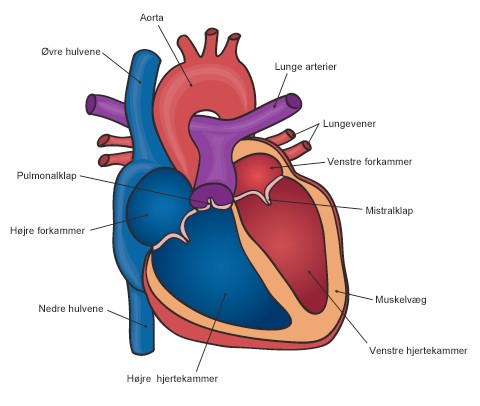
\includegraphics[width=0.5\linewidth]{Teori/Fysiologi/hjerte}
	\caption{Figur af hjertets opbygning \cite{Hjerte}}
	\label{fig:hjerte}
\end{figure}

Hjertet består af to halvdele og er adskilt af en kraftig skillevæg. Ud over de to hjertehalvdele
består hjertet også af andre elementer, hér vigtigt at nævne hjerteklapperne, som sørger for,
at blodet kun kan løbe én vej. Hjertet har fire hjerteklapper: To AV-klapper, aortaklappen og
pulmonalklappen. Dette ses også på figur \vref{fig:hjerte}. Hjerteklappernes åbning og lukning bestemmes af trykket på henholdsvis den ene og den anden side. Højre side af hjertet pumper blod ud i lungekredsløbet via lungearterierne, også kaldt det lille kredsløb, mens venstre side af hjertet pumper blod ud i legemskredsløbet via aorta, også kaldt det store kredsløb. Hjertets pumpefunktionen er en vigtig funktion, der har til hovedopgave at transportere blod rundt i kroppen.

For at hjertet kan transportere blodet rundt til hele kroppen kræver det et tryk, der dannes
ved, at hjertet trækker sig sammen med jævne mellemrum. Når hjertet slapper af, er blodtrykket
lavest - denne fase i hjertets cyklus kaldes diastolen, deraf kommer det diastoliske blodtryk. Når
hjertet i stedet kontraherer sig er blodtrykket højst - denne fase i hjertets cyklus kaldes systolen,
deraf kommer det systoliske blodtryk. 

\clearpage

\begin{figure}[h!]
	\centering
	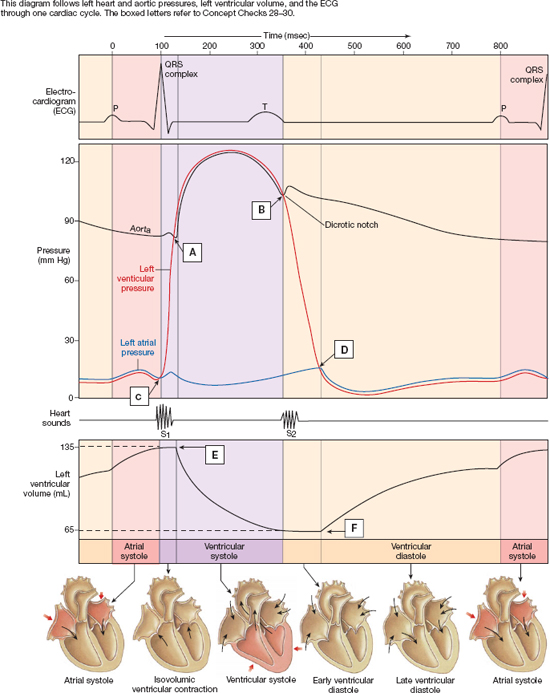
\includegraphics[width=0.9\linewidth]{Teori/Fysiologi/Blodtryk}
	\caption{Wiggers Diagram \cite{WiggersDiagram}}
	\label{fig:blodtryk}
\end{figure}

På figur \vref{fig:blodtryk} ved punkt C ses det, at systolen starter, når trykket i ventriklerne overstiger trykket i arterierne. AV-klapperne lukkes for at forhindre tilbagestrømning af blodet. Når trykket i venstre ventrikel overstiger trykket i aorta åbnes aortaklappen og blodet vil strømme ud, dette ses ved punkt A. Ved punkt E ses det, at volumenet i ventriklerne falder, idet blodet løber fra ventriklen til aorta, og videre ud i det store kredsløb som tidligere nævnt. 

På figur \vref{fig:blodtryk} ved punkt D ses det, at diastolen starter, når trykket i ventriklerne er lavere end i arterierne. Dette medfører, at den ene AV-klap åbnes, som det ses ved punkt B, så hjertet kan fyldes med blod. Under diastolen er aortaklappen lukket. Ved punkt F ses det, at volumenet i ventriklerne stiger, idet blodet løber fra atrierne til ventriklerne. 

Blodtrykket måles som det tryk, der er højere end det atmosfæriske tryk. Det angives normalvis i mmHg

Blodtryk kan måles invasivt eller non-invasivt. Da det er givet i problemformuleringen, at vi skal vise blodtrykket som funktion af tiden, dvs. det skal vises kontinerligt, vil dette projekt omhandle et invasivt blodtryksmålesystem. 




	\documentclass[a4paper,11pt,fleqn,oneside,openany]{memoir} 	% Openright aabner kapitler paa hoejresider (openany begge)

\reparticle 
\chapterstyle{hangnum} 
\hangsecnum

%%%% PACKAGES %%%%
% section font size
%\usepackage{titlesec}
%\titleformat*{\section}{\LARGE\bfseries}

% ¤¤ Oversaettelse og tegnsaetning ¤¤ %
\usepackage[utf8x]{inputenc}					% Input-indkodning af tegnsaet (UTF8)
\usepackage[danish]{babel}					% Dokumentets sprog
\usepackage[T1]{fontenc}					% Output-indkodning af tegnsaet (T1)
\usepackage{ragged2e,anyfontsize}			% Justering af elementer
%\usepackage{fixltx2e}						% Retter forskellige fejl i LaTeX-kernen
\setaftersubsubsecskip{1pt}	
\setaftersubsecskip{1pt}
\setbeforesubsecskip{-\baselineskip}
\setaftersecskip{1pt}
\setbeforesecskip{1ex}
\setaftersecskip{1ex}


\usepackage{textcomp}
																		
% ¤¤ Figurer og tabeller (floats) ¤¤ %
\usepackage{graphicx} 						% Haandtering af eksterne billeder (JPG, PNG, PDF)
\usepackage{multirow}                		% Fletning af raekker og kolonner (\multicolumn og \multirow)
\usepackage{colortbl} 						% Farver i tabeller (fx \columncolor, \rowcolor og \cellcolor)
\usepackage[dvipsnames]{xcolor}				% Definer farver med \definecolor. Se mere: 			
											% http://en.wikibooks.org/wiki/LaTeX/Color
									
\usepackage{flafter}						% Soerger for at floats ikke optraeder i teksten foer deres reference
\let\newfloat\relax 						% Justering mellem float-pakken og memoir
\usepackage{float}							% Muliggoer eksakt placering af floats, f.eks. \begin{figure}[H]
%\usepackage{eso-pic}						% Tilfoej billedekommandoer paa hver side
\usepackage{wrapfig}						% Indsaettelse af figurer omsvoebt af tekst. \begin{wrapfigure}{Placering}{Stoerrelse}
%\usepackage{multicol}         	        	% Muliggoer tekst i spalter
%\usepackage{rotating}						% Rotation af tekst med \begin{sideways}...\end{sideways}
\usepackage{longtable}						%Muliggør at lange tabeller deler sig over flere sider (Det gør de ikke med table eller tabular)
\usepackage{hhline}							%Dobbeltlinjer både vertikalt og horisontalt i tabeller.
\usepackage{xr}								%Referace til andet dokument

% Opsætning af farver i chapter/sections mm.

\definecolor{chaptercolor}{gray}{0.5}		% Definerer en farve til brug til kapiteludseende
\newif\ifchapternonum

\renewcommand\thechapter{\color{RoyalBlue}\arabic{chapter}}
\renewcommand\thesection{\textcolor{RoyalBlue}{\thechapter.}\color{RoyalBlue}\arabic{section}}



% ¤¤ Matematik mm. ¤¤
\usepackage{amsmath,amssymb,stmaryrd} 		% Avancerede matematik-udvidelser
\usepackage{mathtools}						% Andre matematik- og tegnudvidelser
\usepackage{textcomp}                 		% Symbol-udvidelser (f.eks. promille-tegn med \textperthousand )
\usepackage{siunitx}						% Flot og konsistent praesentation af tal og enheder med \si{enhed} og \SI{tal}{enhed}
\sisetup{output-decimal-marker = {,}}		% Opsaetning af \SI (DE for komma som decimalseparator) 
\usepackage[version=3]{mhchem} 				% Kemi-pakke til flot og let notation af formler, f.eks. \ce{Fe2O3}
%\usepackage{rsphrase}						% Kemi-pakke til RS-saetninger, f.eks. \rsphrase{R1}

\usepackage{tabularx}

% ¤¤ Referencer og kilder ¤¤ %
\usepackage[danish]{varioref}				% Muliggoer bl.a. krydshenvisninger med sidetal (\vref)
\usepackage{natbib}							% Udvidelse med naturvidenskabelige citationsmodeller
%\bibliographystyle{plain}					% Referencestilen. kan bruges: abbrvnat, ksfh_nat, plain
%\usepackage{cite}
%\usepackage{citeall}
%\setcitestyle{longnamefirst,open={((},close={))}}
%\usepackage{xr}							% Referencer til eksternt dokument med \externaldocument{<NAVN>}
%\usepackage{glossaries}					% Terminologi- eller symbolliste (se mere i Daleifs Latex-bog)

% ¤¤ Misc. ¤¤ %
\usepackage{listings}						% Placer kildekode i dokumentet med \begin{lstlisting}...\end{lstlisting}
\usepackage{lipsum}							% Dummy text \lipsum[..]
\usepackage[shortlabels]{enumitem}			% Muliggoer enkelt konfiguration af lister
\usepackage{pdfpages}						% Goer det muligt at inkludere pdf-dokumenter med kommandoen \includepdf[pages={x-y}]{fil.pdf}	
\pdfoptionpdfminorversion=6					% Muliggoer inkludering af pdf dokumenter, af version 1.6 og hoejere
\pretolerance=2500 							% Justering af afstand mellem ord (hoejt tal, mindre orddeling og mere luft mellem ord)

% Kommentarer og rettelser med \fxnote. Med 'final' i stedet for 'draft' udloeser hver note en error i den faerdige rapport.
\usepackage[footnote,draft,danish,silent,nomargin]{fixme}		


%%%% CUSTOM SETTINGS %%%%

% ¤¤ Marginer ¤¤ %
\setlrmarginsandblock{2.5cm}{2.5cm}{*}		% \setlrmarginsandblock{Indbinding}{Kant}{Ratio}
\setulmarginsandblock{2.5cm}{2.5cm}{*}		% \setulmarginsandblock{Top}{Bund}{Ratio}
\checkandfixthelayout 						% Oversaetter vaerdier til brug for andre pakker

%	¤¤ Afsnitsformatering ¤¤ %
\setlength{\parindent}{0mm}           		% Stoerrelse af indryk
\setlength{\parskip}{3mm}          			% Afstand mellem afsnit ved brug af double Enter
\linespread{1,1}							% Linie afstand

% ¤¤ Litteraturlisten ¤¤ %
\bibpunct[,]{[}{]}{;}{n}{,}{,} 				% Definerer de 6 parametre ved Harvard henvisning (bl.a. parantestype og seperatortegn)
\bibliographystyle{unsrtnat}			% Udseende af litteraturlisten. bibtex/harvard, unsrt, unsrtnat, agsm


% ¤¤ Indholdsfortegnelse ¤¤ %
\setsecnumdepth{subsubsection}		 				% Dybden af nummerede overkrifter (part/chapter/section/subsection)
\maxsecnumdepth{subsubsection}					% Dokumentklassens graense for nummereringsdybde
\settocdepth{subsection} 					% Dybden af indholdsfortegnelsen

% ¤¤ Lister ¤¤ %
\setlist{
  topsep=0pt,								% Vertikal afstand mellem tekst og listen
  itemsep=-1ex,								% Vertikal afstand mellem items
} 

% ¤¤ Visuelle referencer ¤¤ %
\usepackage[hyphens]{url}
\usepackage[colorlinks]{hyperref}			% Danner klikbare referencer (hyperlinks) i dokumentet.
\hypersetup{colorlinks = true,				% Opsaetning af farvede hyperlinks (interne links, citeringer og URL)
    linkcolor = black,
    citecolor = black,
    urlcolor = black
}

% ¤¤ Opsaetning af figur- og tabeltekst ¤¤ %
\captionnamefont{\small\bfseries\itshape}	% Opsaetning af tekstdelen ('Figur' eller 'Tabel')
\captiontitlefont{\small}					% Opsaetning af nummerering
\captiondelim{. }							% Seperator mellem nummerering og figurtekst
\hangcaption								% Venstrejusterer flere-liniers figurtekst under hinanden
\captionwidth{\linewidth}					% Bredden af figurteksten
\setlength{\belowcaptionskip}{0pt}			% Afstand under figurteksten
		
% ¤¤ Opsaetning af listings ¤¤ %
%\setmonofont{Consolas} %to be used with XeLaTeX or LuaLaTeX
\definecolor{bluekeywords}{rgb}{0,0,1}
\definecolor{greencomments}{rgb}{0,0.5,0}
\definecolor{redstrings}{rgb}{0.64,0.08,0.08}
\definecolor{xmlcomments}{rgb}{0.5,0.5,0.5}
\definecolor{types}{rgb}{0.17,0.57,0.68}
\definecolor{turquoise}{rgb}{0.0, 0.81, 0.82}

\usepackage{listings}
\lstset{language=[Sharp]C,
	captionpos=b,
	numbers=left, %Nummerierung
	numberstyle=\tiny, % kleine Zeilennummern
	frame=lines, % Oberhalb und unterhalb des Listings ist eine Linie
	showspaces=false,
	showtabs=false,
	breaklines=true,
	showstringspaces=false,
	breakatwhitespace=true,
	escapeinside={(*@}{@*)},
	commentstyle=\color{greencomments},
	morekeywords={partial, var, value, get, set},
	morekeywords=[2]{Test, Assert, Is},
	keywordstyle=\color{bluekeywords},
	keywordstyle={[2]\color{turquoise}},
	stringstyle=\color{redstrings},
	basicstyle=\ttfamily\small,
	tabsize=2
}


%\definecolor{commentGreen}{RGB}{34,139,24}
%\definecolor{stringPurple}{RGB}{208,76,239}

%\lstset{language=[Sharp]C,					% Sprog
%	basicstyle=\ttfamily\scriptsize,		% Opsaetning af teksten
%	keywords={for,if,while,else,elseif,		% Noegleord at fremhaeve
%			  end,break,return,case,
%			  switch,function},
%	keywordstyle=\color{blue},				% Opsaetning af noegleord
%	commentstyle=\color{commentGreen},		% Opsaetning af kommentarer
%	stringstyle=\color{stringPurple},		% Opsaetning af strenge
%	showstringspaces=false,					% Mellemrum i strenge enten vist eller blanke
%	numbers=left, numberstyle=\tiny,		% Linjenumre
%	extendedchars=true, 					% Tillader specielle karakterer
%	columns=flexible,						% Kolonnejustering
%	breaklines, breakatwhitespace=true		% Bryd lange linjer
%}

% ¤¤ Navngivning ¤¤ %
\addto\captionsdanish{
	\renewcommand\appendixname{Appendiks}
	\renewcommand\contentsname{Indholdsfortegnelse}	
	\renewcommand\appendixpagename{Appendiks}
	\renewcommand\appendixtocname{Appendiks}
	%\renewcommand\cftchaptername{\chaptername~}
	\renewcommand\cftchaptername{\color{RoyalBlue}Kapitel }
					% Skriver "Kapitel" foran kapitlerne i indholdsfortegnelsen
	\renewcommand\cftappendixname{\appendixname~}			% Skriver "Appendiks" foran appendiks i indholdsfortegnelsen
}

% ¤¤ Kapiteludsende ¤¤ %

\makechapterstyle{jenor}{					% Definerer kapiteludseende frem til ...
  \renewcommand\beforechapskip{0pt}
  \renewcommand\printchaptername{}
  \renewcommand\printchapternum{}
  \renewcommand\printchapternonum{\chapternonumtrue}
  \renewcommand\chaptitlefont{\fontfamily{bch}\fontseries{m}\fontshape{ol}\fontsize{30}{35}\selectfont\raggedright\selectfont\color{chaptercolor}}
  \renewcommand\chapnumfont{\fontfamily{bch}\fontseries{m}\fontshape{n}\fontsize{1in}{0in}\selectfont\raggedleft\selectfont\color{RoyalBlue}}
  \renewcommand\printchaptertitle[1]{%
    \noindent
    \ifchapternonum
    \begin{tabularx}{\textwidth}{X}
    {\let\\\newline\chaptitlefont ##1\par} 
    \end{tabularx}
%    \par\vskip-2.5mm\hrule
    \else
    \begin{tabularx}{\textwidth}{Xl}
    	
    \raisebox{-15pt}{\chapnumfont \thechapter} & {\hspace{2.5cm}\parbox[b]{\linewidth}{\chaptitlefont ##1}}
    
    \end{tabularx}
%    \par\vskip2mm\hrule
    \fi
  }
}											% ... her



\chapterstyle{jenor}						% Valg af kapiteludseende - Google 'memoir chapter styles' for alternativer

% ¤¤ Sidehoved ¤¤ %

\makepagestyle{Uni}							% Definerer sidehoved og sidefod udseende frem til ...
\makepsmarks{Uni}{%
	\createmark{chapter}{left}{shownumber}{}{. \ }
	\createmark{section}{right}{shownumber}{}{. \ }
	\createplainmark{toc}{both}{\contentsname}
	\createplainmark{lof}{both}{\listfigurename}
	\createplainmark{lot}{both}{\listtablename}
	\createplainmark{bib}{both}{\bibname}
	\createplainmark{index}{both}{\indexname}
	\createplainmark{glossary}{both}{\glossaryname}
}
\nouppercaseheads											% Ingen Caps oenskes

\makeevenhead{Uni}{}{}{\leftmark}				% Definerer lige siders sidehoved (\makeevenhead{Navn}{Venstre}{Center}{Hoejre})
\makeoddhead{Uni}{\rightmark}{}{Ingeniørhøjskolen Aarhus Universitet}			% Definerer ulige siders sidehoved (\makeoddhead{Navn}{Venstre}{Center}{Hoejre})
\makeevenfoot{Uni}{}{}{Side \thepage{} af \thelastpage}							% Definerer lige siders sidefod (\makeevenfoot{Navn}{Venstre}{Center}{Hoejre})
\makeoddfoot{Uni}{}{}{Side \thepage{} af \thelastpage}								% Definerer ulige siders sidefod (\makeoddfoot{Navn}{Venstre}{Center}{Hoejre})
\makeheadrule{Uni}{\textwidth}{0.5pt}						% Tilfoejer en streg under sidehovedets indhold
\makefootrule{Uni}{\textwidth}{0.5pt}{1mm}					% Tilfoejer en streg under sidefodens indhold

\copypagestyle{Unichap}{Uni}								% Sidehoved for kapitelsider defineres som standardsider, men med blank sidehoved
\makeoddhead{Unichap}{}{}{}
\makeevenhead{Unichap}{}{}{}
\makeheadrule{Unichap}{\textwidth}{0pt}
\aliaspagestyle{chapter}{Unichap}							% Den ny style vaelges til at gaelde for chapters
															% ... her
															
\pagestyle{Uni}												% Valg af sidehoved og sidefod (benyt "plain" for ingen sidehoved/fod)


%%%% CUSTOM COMMANDS %%%%

% ¤¤ Billede hack ¤¤ %										% Indsaet figurer nemt med \figur{Stoerrelse}{Fil}{Figurtekst}{Label}
\newcommand{\figur}[4]{
		\begin{figure}[H] \centering
			\includegraphics[width=#1\textwidth]{billeder/#2}
			\caption{#3}\label{#4}
		\end{figure} 
}

% ¤¤ Specielle tegn ¤¤ %
\newcommand{\decC}{^{\circ}\text{C}}
\newcommand{\dec}{^{\circ}}
\newcommand{\m}{\cdot}


%%%% ORDDELING %%%%

\hyphenation{}



\begin{document}
	\thispagestyle{empty}
\newcommand{\HRule}{\rule{\linewidth}{0.1mm}} % Defines a new command for the horizontal lines, change thickness here

\begin{center}
	\vspace{5cm}
	
	\begin{figure}[h!]
		\centering
		
\includegraphics[width=0.5\linewidth]{Forside/AUlogo}
	\end{figure}
	
	\vspace{0.1 in}
	%\textsc{\LARGE Ingeniørhøjskolen Aarhus Universitet}\\[1.5cm] %
	
	\textsc{\large 3. Semester projekt \\Accepttest}\\[1.5cm] 
	
	\HRule \\[0.8cm]
	{\huge \bfseries \textsc{Udvikling af et blodtrykmålesystem}} 
	
	{\LARGE Accepttest} \\[0.4cm]
	\HRule \\[1.5cm]
	
	
	
	
	\vspace{0.2 in}
	\begin{center}
		\begin{tabular}{l c r}
			\textbf{Navn} & \textbf{AU ID} & \textbf{Studienummer} \\
			Caroline Kaagaard Dahl Laursen & \textsl{AU572444} & \textsl{201611025}  \\
			Nicolai Bæch & \textsl{AU580049} & \textsl{201704646}  \\
			Mathias Egsgaard & \textsl{AU590400} & \textsl{201705031}  \\
			Thea Plenus Kjeldahl Kristensen & \textsl{AU577124} & \textsl{201707180}  \\
			Sarah Krohn Fenger & \textsl{AU577425} & \textsl{201707931}  \\
			Mikkel Rugholm Boisen & \textsl{AU578833} & \textsl{201708119}  \\
			Kajene Elankanathan & \textsl{AU594051} & \textsl{201710472}  \\
			
			
		\end{tabular}
	\end{center}
	\vspace{0.5 in}
	
	\textsc{\large Vejleder: Samuel Alberg Thrysøe}
	\vspace{0.5 in}
	
	\textsc{\large Dato: 19/12-2018}\\
	\vspace{0.5 in}
	
	
	\textsc{Antal sider: xx} \\
	%{\large\textit{\today}} \\[3cm]
	\vfill % Fill the rest of the page with whitespace
	
\end{center} % Center everything on the page

\clearpage

\newpage
	\chapter*{Versionshistorik}

\begin{table}[h!]
	\begin{tabular}{l|l|l|l}
		{\color[HTML]{187ABD} \textbf{Version}} & {\color[HTML]{187ABD} \textbf{Dato}} & {\color[HTML]{187ABD} \textbf{Initialer}} & {\color[HTML]{187ABD} \textbf{Beskrivelse}} \\ \hline
		0.1 & {\color[HTML]{000000} 04-09-2018} & KE & Oprettelse af dokument "Accepttest" \\ \hline
		0.2 & 16-09-2018 & TPKK & Tilføjelse af indholdsfortegnelse og overskrifter \\ \hline
		0.3 & 16-09-2018 & KE & Rettelse af "Ikke-funktionelle krav" \\ \hline
		0.4 & 24-09-2018 & CKDL & Rettelse af UC1 og UC2 \\ \hline
		0.5 & 30-09-2018 & SKF & Rettelser \\ \hline
		1.0 & 06-12-2018 & TPKK & Rettelse af UC5 \\ \hline
		1.1 & 13-12-2018 & SKF & Rettelser efter Accepttest med vejleder \\ \hline
		2.0 & 14-12-2018 & CKDL & Opstilling af endeligt dokument "Accepttest" i LaTex
	\end{tabular}
\end{table}

\clearpage
	\chapter*{Godkendelsesformular}

\begin{table}[h!]
	\begin{tabular}{|l|llllllllllllllllllllllllllll|}
		\hline
		\textbf{Forfatter(e):} &  &  &  &  &  &  &  &  &  &  &  &  &  &  &  &  &  &  &  &  &  &  &  &  &  &  &  &  \\
		&  &  &  &  &  &  &  &  &  &  &  &  &  &  &  &  &  &  &  &  &  &  &  &  &  &  &  &  \\
		\hline
		\textbf{Godkendes af:} &  &  &  &  &  &  &  &  &  &  &  &  &  &  &  &  &  &  &  &  &  &  &  &  &  &  &  &  \\
		&  &  &  &  &  &  &  &  &  &  &  &  &  &  &  &  &  &  &  &  &  &  &  &  &  &  &  &  \\
		\hline
		\textbf{Projektnummer:} &  &  &  &  &  &  &  &  &  &  &  &  &  &  &  &  &  &  &  &  &  &  &  &  &  &  &  &  \\
		&  &  &  &  &  &  &  &  &  &  &  &  &  &  &  &  &  &  &  &  &  &  &  &  &  &  &  &  \\
		\hline
		\textbf{Dokument-ID:} &  &  &  &  &  &  &  &  &  &  &  &  &  &  &  &  &  &  &  &  &  &  &  &  &  &  &  &  \\
		&  &  &  &  &  &  &  &  &  &  &  &  &  &  &  &  &  &  &  &  &  &  &  &  &  &  &  &  \\
		\hline
		\textbf{Antal sider:} &  &  &  &  &  &  &  &  &  &  &  &  &  &  &  &  &  &  &  &  &  &  &  &  &  &  &  &  \\
		&  &  &  &  &  &  &  &  &  &  &  &  &  &  &  &  &  &  &  &  &  &  &  &  &  &  &  &  \\
		\hline
		\textbf{Kunde:} &  &  &  &  &  &  &  &  &  &  &  &  &  &  &  &  &  &  &  &  &  &  &  &  &  &  &  &  \\
		&  &  &  &  &  &  &  &  &  &  &  &  &  &  &  &  &  &  &  &  &  &  &  &  &  &  &  & \\
		\hline
	\end{tabular}
\end{table}

\vspace{1 cm}
Ved underskrivelse af dette dokument accepteres det af begge parter, som værende kravende til det ønskede system
\vspace{1.5 cm}

\begin{table}[h!]
	\begin{tabular}{@{}p{2.5in}@{}}
		\hrulefill \\
		Dato 
	\end{tabular} \hfill
	\quad
	\begin{tabular}{@{}p{2.5in}@{}}
		\hrulefill \\
		Sted \\
	\end{tabular}
\end{table}

\vspace{1 cm}

\begin{table}[h!]
	\begin{tabular}{@{}p{2.5in}@{}}
		\hrulefill \\
		<Kunde underskrift> 
	\end{tabular} \hfill
	\quad
	\begin{tabular}{@{}p{2.5in}@{}}
		\hrulefill \\
		<Leverandør underskrift> \\
	\end{tabular}
\end{table}


\clearpage


	
		\begin{KeepFromToc}
			\tableofcontents
		\end{KeepFromToc}
	
	\chapter{Ordliste}

\begin{table}[h!]
	\begin{tabular}{l|l}
		\textbf{Ord} & \textbf {Forklaring} \\ 
		\hline
		TPKK & Thea Plenus Kjeldahl Kristensen \\
		\hline
		SKF & Sarah Krohn Fenger \\
		\hline
		CKDL & Caroline Kaagaard Dahl Laursen \\
		\hline
		KE & Kajene Elankanathan \\
		\hline
		UC & Use Case \\
		\hline
		GUI & Graphical User Interface \\
		\hline
		Ext & Extension \\
		\hline
		VS & Microsoft Visual Studio \\
		\hline
		CPR & Centrale personregister \\
		\hline
		 &  \\
		\hline
		 &  \\
		\hline
		 &  \\
		\hline
		 &  \\
		\hline
	\end{tabular}
	\caption{Ordliste}
	\label{table:Ordliste}
\end{table}

\clearpage
	%\chapter*{Læsevejledning}
I denne rapport redegøres for valgene bag arkitekturen og designet til Rambøll Tilsyn. 

Arkitektur og design dokumentationen kan overordnet inddeles i 2 sektioner:\\
Første sektion er en beskrivelse af arkitekturen for systemet.

I anden sektion er der en beskrivelse af designvalgene til henholdvis Firebase og Rambøll Tilsyn.

I slutningen af rapporten  findes ordforklaring og litteraturliste.

	%\chapter{Problemformulering}

\section{Projektformulering}
Projektet har til formål at udvikle en prototype af et blodtryks målesystem, der kan måle, behandle og visualisere blodtryk og puls. Systemet er udviklet med henblik på hurtigt at kunne advare brugeren om et eventuelt fald- eller stigning i blodtryk eller puls.

Det udviklede system kan:

\begin{itemize}
	\item Måle blodtryk på en patient
	\item Visualisere det målte blodtryk kontinuert ved hjælp af en graf på en brugergrænseflade
	\item Visualisere det målte blodtryk i form af tal på en brugergrænseflade, herunder systolisk-, diastolisk- samt median blodtryk
	\item Beregne patientens puls
	\item Visualisere den beregnede puls i form af tal på en brugergrænseflade
	\item Alarmere ved: Fejl i nulpunktsjustering, tid til kalibrering, fald- eller stigning i blodtryk, fald- eller stigning i puls samt ved mislykket forsøg på at gemme opsamlet data
	\item Gemme data, herunder blodtryk og puls under patientens CPR-nummer.
	
\end{itemize}

Et færdigudviklet system vil være ideelt til brug på operationsstuer da systemets alarmerings funktion muliggør hurtige reaktioner ved eventuelle fald- eller stigninger i patientens blodtryk, eksempelvis et markant fald i forbindelse med en større blødning.\\


\section{Problemformulering}

Ved måling af blodtryk skelnes mellem systolisk- og diastolisk blodtryk. Hvordan er det muligt ved brug af en tryktransducer at måle dette blodtryk?

Hvordan er det muligt at udvikle et program, der kan illustrere det målte blodtryk kontinuert ved hjælp af en graf samtidig med, at talværdien for henholdsvis det systoliske- og diastoliske afbildes på brugergrænsefladen? Kan det ydermere lade sig gøre at bestemme en patients puls ud fra det målte blodtryk?

Hvad gør en brugergrænseflade god og overskuelig? Hvordan kan man ved en god brugergrænseflade let og overskueligt nemt aflæse de interessante værdier samtidig med, at programmet er nemt at bruge?\clearpage






 





	\section{Systembeskrivelse}
Formålet med dette projekt er at udvikle en invasiv blodtryksmåler, der skal være på en operationsstue. Den invasive blodtryksmåler er et system, der har til formål at kunne måle, angive og visualisere en patients systolisk-, diastolisk og middelblodtryk samt puls. Blodtrykket visualiseres kontinuert, når det tilsluttes det væskefyldte kateter. Derudover vil systemet alarmere i visse situationer beskrevet i punkt 2.2.
Systemet består af en hardware del og en software del. 


Systemets software del skal udvikle et program, der skal kunne kalibrere, vise blodtrykket kontinuerligt, måle puls og gemme de målte data. Derudover skal programmet indeholde et digital filter til filtrering af boldtrykket. Det digitale filter skal kunne slås til og fra. Programmet er bygget op omkring et Graphical User Interface (GUI) bestående af følgende elementer:
\vspace{0.7 cm}

\begin{enumerate}[2.1.]
	\item Knap “Lav nulpunktsjustering” - Laver nulpunktsjustering
	\item Knap “Start” - Påbegynder målingen
	\item Knap “Indstil grænseværdi” - Gør det muligt at ændre på grænseværdier under en måling eller før en måling Pr. deafult er der valgt flg. værdier: 
	Puls øvre: 120
	Puls nedre: 60
	Blodtrykkets øvre grænseværdi er værdien for det systoliske blodtryk. Dette er valgt til 160. 
	Blodtrykkets nedre grænseværdi er værdien for det diastoliske blodtryk. Dette er valgt til 60 
	\item Knap “Ryd” - Rydder alle værdier på brugergrænsefladen
	\item Knap “Stop” - Stopper målingen.
	\item Knap “Gem” - Gemmer værdier for blodtryksmåling, alarmer, digitaltfilter, patientens CPR og brugerens ID.
	\item Knap “Kalibrering” - Kalibrerer systemet.
	\item Knap “Mute alarm” - Gør alarm lydløs. De visuelle effekter vil stadig være synlige.
	\item Knap “Afbryd alarm” - Stopper en alarm.
	\item To radiobuttons - Slår digitalt filter til eller fra. Er monitor valgt er filteret aktiveret. Er mode valgt er filteret deaktiveret. Monitor valgt pr. default. 
	\item Tekstbokse - Indeholder data I form af systolisk-, diastolisk-, middelblodtryk og puls. 
	\item Chart - Indeholder kontinuert graf over patientens blodtryk
\end{enumerate}

\vspace{0.7 cm}
Se også punkt 2.3 “Skitse af brugergrænseflade”


Systemets hardware består af et elektrisk kredsløb der skal kunne forstærke blodtrykssignalet fra en tryktransducer. Før signalet sendes til en AD-converter filtreres det af et analogt antialiaseringsfilter. AD-converterens funktion er at konvertere det analoge signal til et digitalt signal, som vores software kan analysere.

Blodtrykket måles invasivt hvilket betyder, at blodtryksmåleren er tilsluttet patientens arterier via et væskefyldt kateter. Tryktransduceren har en membran, som registrerer trykket vha. stræk modstande. Dog vil vi i vores praktiske situation bruge en væskesøjle til at agere som patient. 


Når systemets opsætning er klart, trykkes der på “start”-knappen, som igangsætter signalvejen gennem hardwaren og ind på GUI'en. Herpå vil talværdierne svarende til patients værdier blive præsenteret. Sker der et fald i blodtrykket, f.eks. I forbindelse med en operation, vil systemet registrere dette, og starte en alarm, således brugeren gøres opmærksomme på et fald i blodtrykket. Alarmen startes, når blodtrykket falder under eller overstiger grænseværdierne, hvor det diastoliske blodtryk er den nedre grænseværdi, og det systoliske blodtryk er den øvre grænseværdi.  


Brugeren kan stoppe alarmen eller slå lyden fra alarmen, samt stoppe målingen. Efter brugeren har foretaget en blodtryksmåling, gemmes blodtryksmålingens værdier, patientens CPR-nummer, digitalt filter, alarmer og brugerens ID-nummer.
\vspace{0.9 cm}
\section{Beskrivelse af alarmer}

Systemet skal i henhold til standard 60601-1-8 kunne alarmere ved eventuelle ændringer i blodtryk samt puls. Systemet findes i operationsstuer og brugsscenariet vil derfor typisk være i forbindelse med operationer. Systemet skal alarmere ved:

\begin{enumerate}[2.2.1]
	\item Fald eller stigning i blodtryk ud over de justerbare grænseværdier
	\item Fald eller stigning i puls ud over de justerbare grænseværdier
\end{enumerate}

Alarm 2.2.1 er kategoriseret “high priority” og skal alarmere i henhold til dokumentet “Standard 60601-1-8”. Den er kategoriseret high idet det er livsfarligt for patienten, hvis der ikke handles med det samme.

Alarm 2.2.2 er kategoriseret “high priority” og skal alarmere i henhold til dokumentet “Standard 60601-1-8”. Den er kategoriseret high idet det er livsfarligt for patienten, hvis der ikke handles med det samme.
	\chapter{Funktionelle krav}
\section{Aktør kontekst diagram}

\begin{figure}[h!]
	\centering
	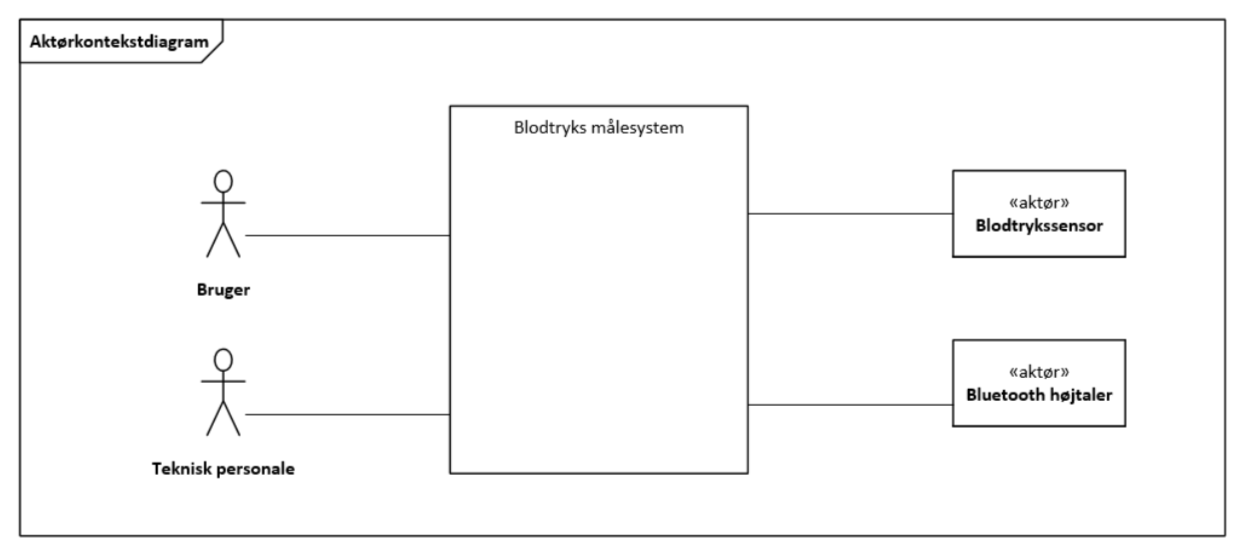
\includegraphics[width=0.5\linewidth]{Kravspecifikation/Aktoer_kontekst_diagram}
\end{figure}
\vspace{1 cm}
\section{Aktørbeskrivelser}
\vspace{0.5 cm}

\begin{longtable}{lllll}
	\hline
	\textbf{Aktør} & \textbf{Type} & \textbf{Beskrivelse} & \textbf{Samtidige forekomster} &  \\ \hline
	\endfirsthead
	%
	\endhead
	%
	\hline
	\endfoot
	%
	\endlastfoot
	%
	Bruger & Primær & \begin{tabular}[c]{@{}l@{}}Brugeren betjener \\ blodtryks målesystemet. \\ Brugeren nulpunkts-\\ justerer, igangsætter og\\ stopper måling. Brugeren \\ er en sundhedsfaglig \\ person, der arbejder på \\ operationsstuen.\end{tabular} & \begin{tabular}[c]{@{}l@{}}1. Da der kun er én \\ blodtryksmåler i \\ systemet, kan der kun \\ være en bruger.\end{tabular} &  \\ \hline
	Teknisk personale & Primær & \begin{tabular}[c]{@{}l@{}}Teknisk personale er \\ teknisk uddannet og \\ skal foretage kalibreringen \\ af systemet.\end{tabular} & \begin{tabular}[c]{@{}l@{}}1. Da der kun er én \\ blodtryksmåler i \\ systemet, kan der kun \\ være et teknisk \\ personale\end{tabular} &  \\
	\hline
	Blodtryksensor & Sekundær & \begin{tabular}[c]{@{}l@{}}Blodtryksensoren er et \\ interface for patienten som \\ er koblet til systemet\end{tabular} & \begin{tabular}[c]{@{}l@{}}1. Da der kun er én \\ blodtryksmåler i \\ systemet, kan der kun \\ være en blodtryksensor\end{tabular} &  \\
	Bluetooth højtaler & Sekundær & \begin{tabular}[c]{@{}l@{}}Bluetooth højtaleren \\ afspiller lyden for de \\ alarmer der står i system-\\ beskrivelsen.\end{tabular} & \begin{tabular}[c]{@{}l@{}}1. Da der kun er én \\ blodtryksmåler i \\ systemet, kan der kun \\ være en bluetooth\\ højtaler\end{tabular} &  \\
	\hline
	Skærm & Sekundær & \begin{tabular}[c]{@{}l@{}}Skærmen bruges til at \\ vise brugergrænsefladen \\ meget større end på \\ computeren. Skærmen \\ gør det nemt og overskueligt \\ for hele personalet at følge \\ med i blodtrykmålingen \\ og de målte værdier af \\ systolisk-, diastolisk-, \\ median blodtryk og puls.\end{tabular} & \begin{tabular}[c]{@{}l@{}}1. Da der kun er én \\ blodtryksmåler i \\ systemet, kan der kun \\ være en skærm\end{tabular} &  \\ \hline \caption{Aktørbeskrivelser}
\end{longtable}

\vspace{0.7 cm}



\section{Use Case beskrivelser}
Dette afsnit giver en kort beskrivelse af systemets Use Cases. Systemet har mange funktioner, herunder måling af puls og blodtryk samt vise det på brugergrænsefladen. Grafen for blodtryk vises kontinuert og værdi for systolisk-, diastolisk-, og median blodtryk samt puls vises i form af tal. Derudover kan systemet alarmere i henhold til punkt 2.2. Systemet kan gemme blodtryksværdierne, digital filter status, brugerens ID-nummer, patientens CPR-nummer, alarmer samt alarmbetingelser. Systemet har endvidere et digitalt filter, som kan slås til og fra på brugergrænsefladen. 
\subsection{Use Case 1: Mål og vis blodtryk og puls}
Formålet med denne use case er få en patients blodtryk visualiseret kontinuerligt samt vise værdierne for patientens systoliske-, diastoliske- og middelblodtryk samt puls. Før brugeren kan igangsætte måling af patientens blodtryk og puls skal der foretages en nulpunktsjustering. Dette gøres i forhold til det atmosfæriske tryk i rummet. Brugeren trykker på “Lav nulpunktsjustering”, hvor efter der laves en nulpunktsjustering. Derefter kan brugeren trykke på “start”, hvorefter målingen startes. Derefter kan brugeren slå det digitale filter til eller fra. Brugeren stopper målingen ved at trykke på “stop”.


\subsection{Use Case 2: Justér grænseværdier}
Formålet med denne use case er at justere grænseværdierne for puls samt systolisk- og diastolisk blodtryk. Der er pr. default valgt grænseværdier for blodtryk og puls som beskrevet i systembeskrivelsen. Hvis forholdene ændrer sig, så er det muligt for brugeren at justere i disse grænseværdier. Dette gøres ved at trykke på knappen “Indstil grænseværdi”, og derefter indtaste de ønskede værdier. 

\subsection{Use Case 3: Alarmering}
Formålet med denne use case er at der udløses en alarm i henhold til, det der er beskrevet i punkt 2.2. Brugeren kan vælge at gøre de auditive alarmer lydløse, eller stoppe alarmen helt. Dette gøres på brugergrænsefladen.
Dato og tid for alarmen, de tilknyttede alarm grænser, alarmbetingelsen, grænseværdierne som blev overskredet og alarmens prioritet logges i henhold til dokumentet “Standard 60601-1-8”.

\subsection{Use Case 4: Gem data}
Formålet med denne use case er at rådata, start- og slut tidspunkt, kalibreringsdato, kalibreringsværdi, nulpunktjusteringsværdi, patientens CPR-nummer og brugerens id gemmes i en fil. Det systoliske-, diastoliske-, middelblodtryk og puls gemmes ikke, da disse kan genskabes ud fra rådataen. Efter brugeren har foretaget en blodtryksmåling kan vedkommende vælge at gemme patientens data ved at trykke på knappen “gem”. Der åbnes et nyt vindue, hvor brugeren skal indtaste patientens CPR-nummer, personale ID og dato med tid. Derefter trykker brugeren på “gem” knappen på det nye vindue. Hvis CPR-nummeret ikke er korrekt, kommer der en besked om at brugeren skal tjekke patientens cpr-nummer. Hvis CPR-nummeret er korrekt trykkes der på “gem” knappen igen. Måligens data i form af systolisk- og diastolisk- blodtryk samt middelblodtrykket og puls gemmes i en fil. Kendes patientens CPR-nummer ikke under operation, evt. i forbindelse med en akut situation indtastes 000000-0000 i stedet for CPR-nummer, når der gemmes data.


\subsection{Use Case 5: Kalibrering}
Formålet med denne use case er at kalibre systemet, således et kendt tryk svarer til en kendt spænding. Kalibrering af systemet skal foretages ca. én gang årligt. En teknisk fagperson har ansvaret for kalibreringen af systemet og kan igangsætte kalibreringen ved at trykke på knappen kalibrering, der ses på brugergrænsefladen i punkt 3 “Skitse af brugergrænseflade”. Herefter foretages der 5 målinger med 5 forskellige trykværdier, som er henholdsvis 10 mmHg, 30 mmHg, 50 mmHg, 75 mmHg og 100 mmHg.

\vspace{1 cm}
\input{FunktionelleKrav/Use_case_diagram/Use_case_diagram}
\section{Use Cases: Fully dressed Use Case beskrivelser}
\input{Use_Cases/Use_Cases/Use_Case_1}
\clearpage
\input{Use_Cases/Use_Cases/Use_Case_2}
\input{Use_Cases/Use_Cases/Use_Case_3}
\clearpage
\input{Use_Cases/Use_Cases/Use_Case_4}
\input{Use_Cases/Use_Cases/Use_Case_5}





	\chapter{Ikke funktionelle krav}
Nedenfor beskrives de ikke-funktionelle krav for systemet. MoSCoW-modellen inddeler kravene for systemet i henholdsvis: Must have, Should have, Could have og Won’t have, for herved at skabe et overblik over de opstillede systemkrav. De enkelte punkters placering i forhold til FURPS+ er angivet i parentes.  FURPS+ står for Functionality, Usability, Reliability, Performance, Supportability, og plusset for begrænsninger i forhold til udformning af systemet.


\section{Must have:}
\begin{enumerate}[4.1]
	\item Systemet skal indeholde et elektronisk kredsløb, som forstærker signalet fra tryktransducere (F)
	\item Systemet skal kunne filtrer signalet fra tryktransduceren med et analogt filter (F)
	\item Systemet skal have en brugergrænseflade (U)
	\item Systemet skal kunne filtrere blodtrykket via et digitalt filter (F)
	\item Systemets GUI skal indeholde elementerne beskrevet under punkt 2.1.  
	\item Systemets GUI skal kunne vise en graf inden for 10 sekunder.(R)
	\item Systemet skal kunne stoppe målingen inden for 5 sekunder.
	\item Systemet skal kunne give alarm i henhold til punkt 2.2(F)
	\item Al data på både tal- og graf-form skal kunne slettes(F)
	\item Systemet skal kunne kalibreres (F,U)
	\item Systemet skal kunne foretage en nulpunktsjustering (F,U)
	\item Systemets GUI skal vise systolisk/diastolisk blodtryk og middelblodstryk som hele tal, og den beregnede puls som decimaltal med maks en decimal. (U)
	\item Systemets GUI skal vise en puls på mellem 30 slag pr. minut og 220 slag pr. minut (P).
	\item Systemets GUI skal alarmere i henhold til punkt 2.2.2, hvis pulsen falder til under 60 slag i minuttet og overstiger 120 slag i minuttet (P)
	\item Systemets GUI skal have et diagram, som indeholder en graf der viser de opsamlede blodtryksdata samt puls (F,U)
	\item Systemet skal have baggrundsbelysning tilpasset brugssituationen. (U)
	\item Systemet skal kunne ses fra 1,5 meters afstand i skarpt sollys af en person uden synshandicap, eller som benytter korrekt korrigerende midler.
	\item Diagrammet samt de viste værdier for puls og middelblodtrykket, samt diastolisk/systolisk blodtryk, skal kunne læses på op til 1,5 meters afstand af person uden synshandicap, eller som benytter korrekt korrigerende midler, og må ikke indeholde farver som påvirker folk med farveblindhed (U)
	\item Systemet skal kunne sample med en frekvens på 1000 Hz (P)
	\item Systemet skal alarmere i henhold til punkt 2.2.1, hvis blodtrykket falder til under 60 diastolisk eller stiger til over 160 diastolisk (P)
	\item Middelblodtrykket skal kunne beregnes og vises på GUI’en (P)
	\item Systemet skal kunne vise en værdi for puls, systolisk-, diastolisk- og middelblodtryk inden for ?? (F)

\section{Should have:}
		\item Systemets værdier samt graf bør kunne læses/ses fra 1 meters afstand for en person med normalt syn. Normal syn defineres som en styrke på maks ±0,5 (U)
	
\section{Could have:}
	\item Systemet kunne gemme de opsamlede blodtryksværdier, digitalt filter, alarmer, alarmbetingelser i en database på baggrund af indtastet CPR-nummer, datoangivelse samt klokkeslæt og ID-nummer. (F, R)
	\item Systemet kunne have et lydsignal ved afsluttet blodtryksmåling. (F, U)
	\item Systemet kunne afbilde EKG-måling i forhold til den viste puls (P)
	\item Systemet kunne have muligheden at åbne og afbilde en ældre gemt fil (P)
	

\section{Won't have:}
	\item Systemet kan ikke vise andet end blodtryksmålingen samt angive puls, diastolisk/systolisk blodtryk (F) 
\end{enumerate}
	\input{Afgraensning/Afgraensning}
	\input{Udviklingsvaerktoejer/Udviklingsvaerktoejer}
	
	\chapter*{Ordforklaring}


	
\clearpage

\end{document}


	\section{Systembeskrivelse}
Formålet med dette projekt er at udvikle en invasiv blodtryksmåler, der skal være på en operationsstue. Den invasive blodtryksmåler er et system, der har til formål at kunne måle, angive og visualisere en patients systolisk-, diastolisk og middelblodtryk samt puls. Blodtrykket visualiseres kontinuert, når det tilsluttes det væskefyldte kateter. Derudover vil systemet alarmere i visse situationer beskrevet i punkt 2.2.
Systemet består af en hardware del og en software del. 


Systemets software del skal udvikle et program, der skal kunne kalibrere, vise blodtrykket kontinuerligt, måle puls og gemme de målte data. Derudover skal programmet indeholde et digital filter til filtrering af boldtrykket. Det digitale filter skal kunne slås til og fra. Programmet er bygget op omkring et Graphical User Interface (GUI) bestående af følgende elementer:
\vspace{0.7 cm}

\begin{enumerate}[2.1.]
	\item Knap “Lav nulpunktsjustering” - Laver nulpunktsjustering
	\item Knap “Start” - Påbegynder målingen
	\item Knap “Indstil grænseværdi” - Gør det muligt at ændre på grænseværdier under en måling eller før en måling Pr. deafult er der valgt flg. værdier: 
	Puls øvre: 120
	Puls nedre: 60
	Blodtrykkets øvre grænseværdi er værdien for det systoliske blodtryk. Dette er valgt til 160. 
	Blodtrykkets nedre grænseværdi er værdien for det diastoliske blodtryk. Dette er valgt til 60 
	\item Knap “Ryd” - Rydder alle værdier på brugergrænsefladen
	\item Knap “Stop” - Stopper målingen.
	\item Knap “Gem” - Gemmer værdier for blodtryksmåling, alarmer, digitaltfilter, patientens CPR og brugerens ID.
	\item Knap “Kalibrering” - Kalibrerer systemet.
	\item Knap “Mute alarm” - Gør alarm lydløs. De visuelle effekter vil stadig være synlige.
	\item Knap “Afbryd alarm” - Stopper en alarm.
	\item To radiobuttons - Slår digitalt filter til eller fra. Er monitor valgt er filteret aktiveret. Er mode valgt er filteret deaktiveret. Monitor valgt pr. default. 
	\item Tekstbokse - Indeholder data I form af systolisk-, diastolisk-, middelblodtryk og puls. 
	\item Chart - Indeholder kontinuert graf over patientens blodtryk
\end{enumerate}

\vspace{0.7 cm}
Se også punkt 2.3 “Skitse af brugergrænseflade”


Systemets hardware består af et elektrisk kredsløb der skal kunne forstærke blodtrykssignalet fra en tryktransducer. Før signalet sendes til en AD-converter filtreres det af et analogt antialiaseringsfilter. AD-converterens funktion er at konvertere det analoge signal til et digitalt signal, som vores software kan analysere.

Blodtrykket måles invasivt hvilket betyder, at blodtryksmåleren er tilsluttet patientens arterier via et væskefyldt kateter. Tryktransduceren har en membran, som registrerer trykket vha. stræk modstande. Dog vil vi i vores praktiske situation bruge en væskesøjle til at agere som patient. 


Når systemets opsætning er klart, trykkes der på “start”-knappen, som igangsætter signalvejen gennem hardwaren og ind på GUI'en. Herpå vil talværdierne svarende til patients værdier blive præsenteret. Sker der et fald i blodtrykket, f.eks. I forbindelse med en operation, vil systemet registrere dette, og starte en alarm, således brugeren gøres opmærksomme på et fald i blodtrykket. Alarmen startes, når blodtrykket falder under eller overstiger grænseværdierne, hvor det diastoliske blodtryk er den nedre grænseværdi, og det systoliske blodtryk er den øvre grænseværdi.  


Brugeren kan stoppe alarmen eller slå lyden fra alarmen, samt stoppe målingen. Efter brugeren har foretaget en blodtryksmåling, gemmes blodtryksmålingens værdier, patientens CPR-nummer, digitalt filter, alarmer og brugerens ID-nummer.
\vspace{0.9 cm}
\section{Beskrivelse af alarmer}

Systemet skal i henhold til standard 60601-1-8 kunne alarmere ved eventuelle ændringer i blodtryk samt puls. Systemet findes i operationsstuer og brugsscenariet vil derfor typisk være i forbindelse med operationer. Systemet skal alarmere ved:

\begin{enumerate}[2.2.1]
	\item Fald eller stigning i blodtryk ud over de justerbare grænseværdier
	\item Fald eller stigning i puls ud over de justerbare grænseværdier
\end{enumerate}

Alarm 2.2.1 er kategoriseret “high priority” og skal alarmere i henhold til dokumentet “Standard 60601-1-8”. Den er kategoriseret high idet det er livsfarligt for patienten, hvis der ikke handles med det samme.

Alarm 2.2.2 er kategoriseret “high priority” og skal alarmere i henhold til dokumentet “Standard 60601-1-8”. Den er kategoriseret high idet det er livsfarligt for patienten, hvis der ikke handles med det samme.
	\chapter{Arkitektur}

\section{Hardwarearkitektur}
I den følgende sektion om hardwarearkitektur beskrives opbygningen af systemet ved brug af sysML. Hardwarearkitekturen indholder diagrammerne BDD og IBD samt en kort forklaring af disse. For ydeligere information om interaktionen i systemet henvises til dokumentet arkitektur og design for flere detaljer. Dette dokument indeholder bloktabel og signaltabel, der fortæller om alle blokke, porte og signaler, der ses i diagrammerne. Yderligere information omkring valg af elementer i systemet findes i dokumentet analyse, som findes i bilaget.

\subsection{BDD}
Et BDD viser opbygningen af et system med brug af blokke. Nedenstående diagram på figur \vref{fig:BDD} viser opbygningen af vores blodtrykssytem, der består af en række forskellige elementer. 

\begin{figure}[h!]
	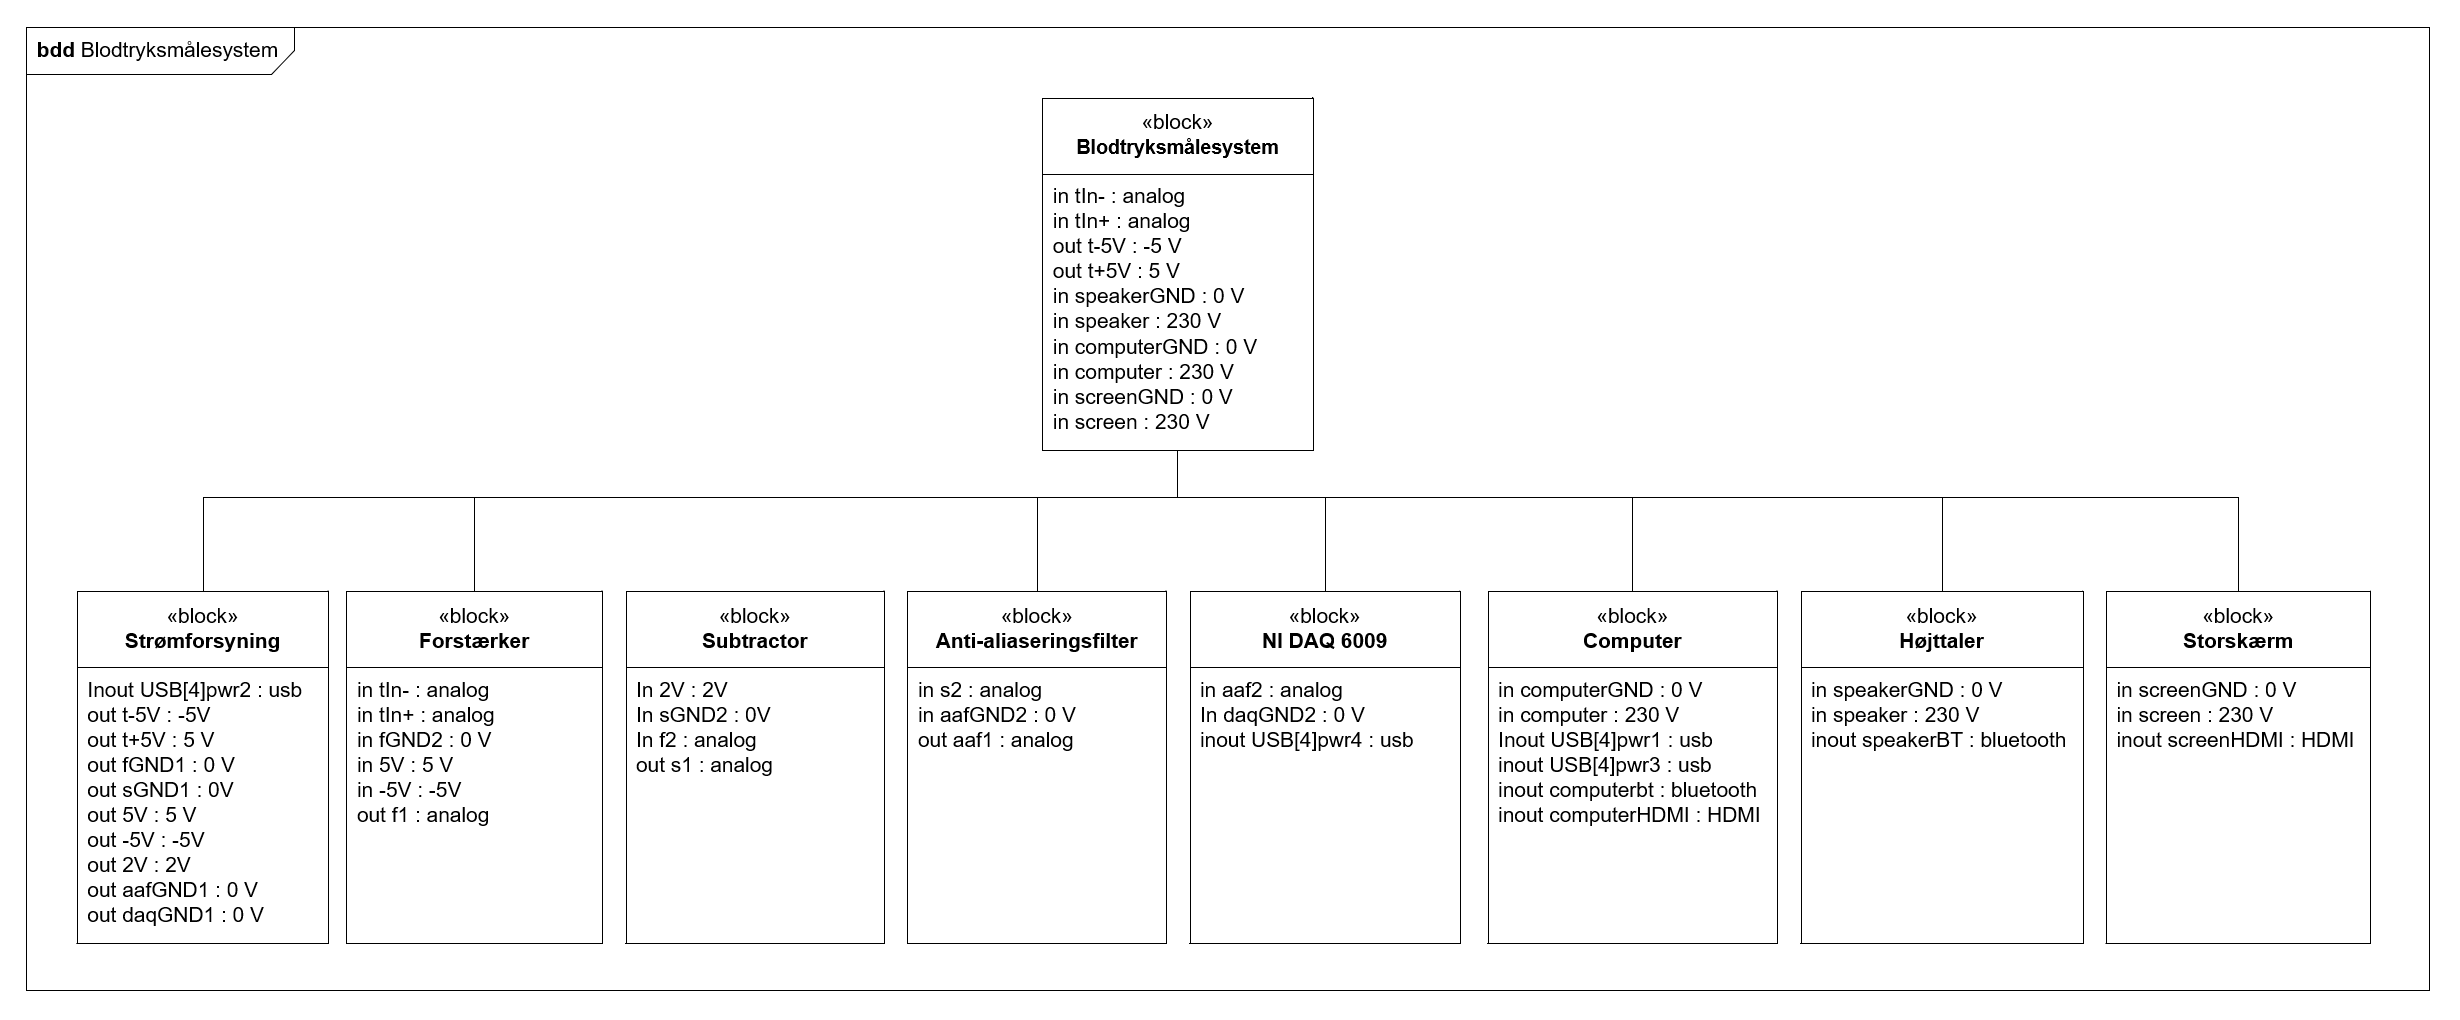
\includegraphics
	[width=1\linewidth]{Arkitektur_og_design/Hardwarearkitektur/BDD_faerdig}
	\caption{BDD Blodtrykmålesystem}
	\label{fig:BDD}
\end{figure}

På BDD'et ses de forskellige elementer, der er er en del af blodtrykmålesystemet. Den øverste blok $"$Blodtryksmålesystem$"$ viser systemets interaktioner med udefrakommende objekter. I denne blok findes tilslutningen til tryktransduceren, som ikke er en del af selve systemet. I blokken findes også tilslutningen af strøm til henholdsvis computer, højtaler og storskærm. 

På diagrammet ses også otte blokke, der repræsenterer de forskellige dele af systemet. Systemet består altså af en strømforsyning, en forstærker, en subtractor, et filter, en AD-Converter, en computer, en højtaler og en storskærm. Strømforsyningen giver strøm til tryktransducer, forstærker og subtractor og udgøres af Analog Discovery. Forstærker, subtractor og filter er designet til systemet i forbindelse med projektet. Mere info om disse elementer i afsnit .... om design af hardware.

\clearpage

\subsection{IBD}
Et IBD viser en mere detaljeret opbygning af et system fordi alle forbindelser mellem blokkene, der findes i BDD'et er tegnet. På nedenstående figur \vref{fig:IBD} ses derved opbygningen af blodtryksmålesystemet inklusiv alle forbindelser mellem blokkene.

\begin{figure}[h!]
	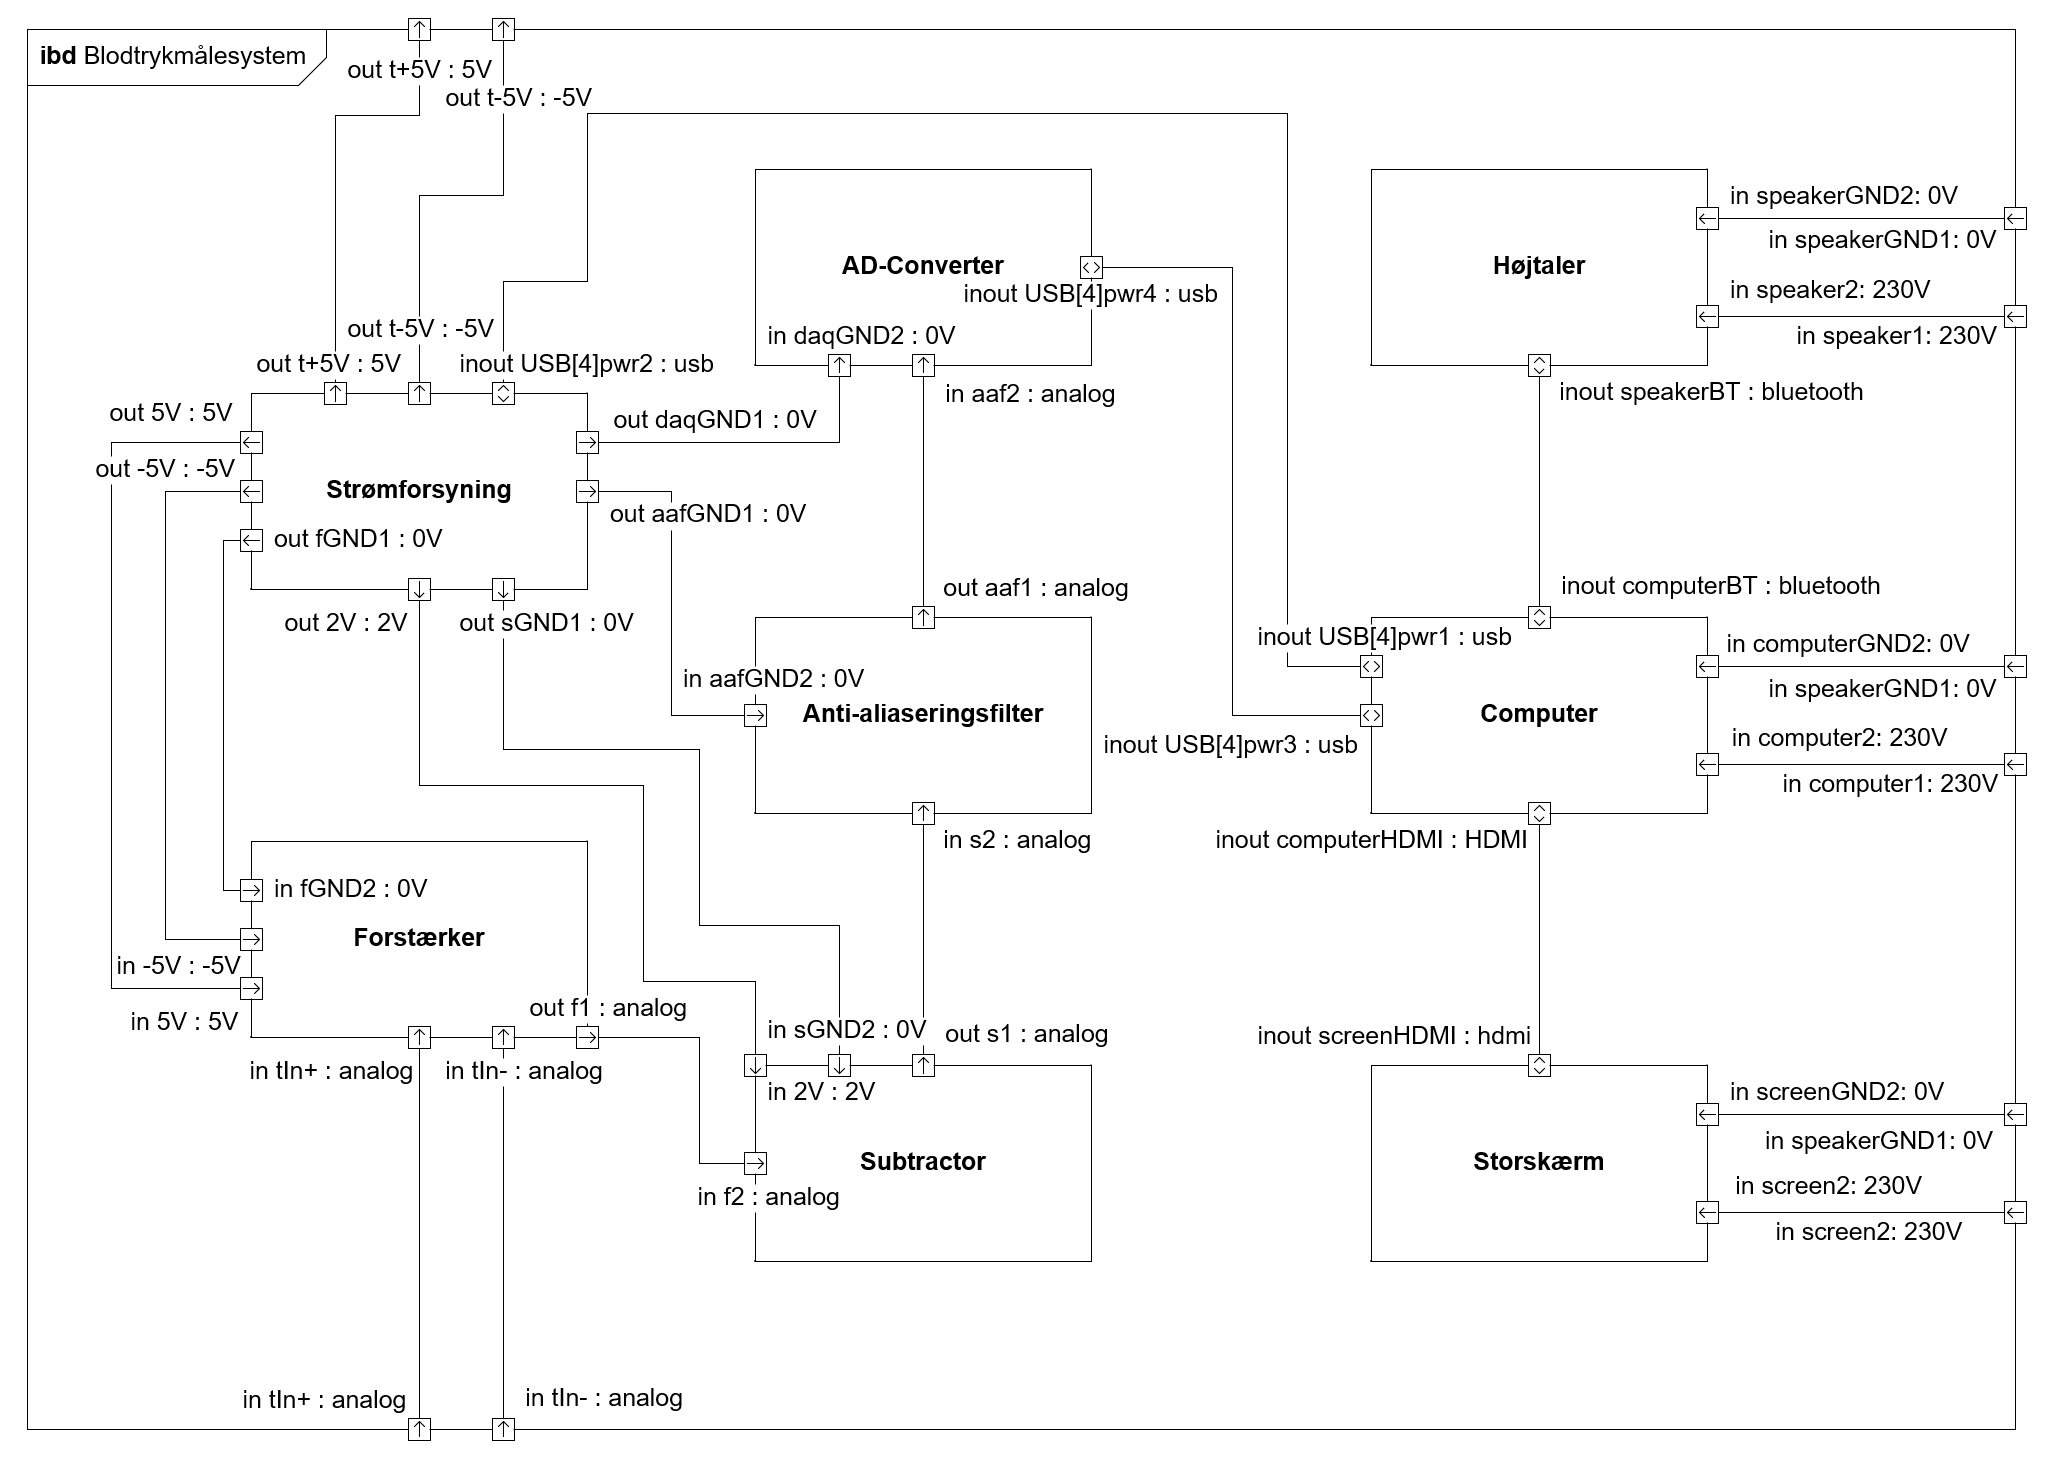
\includegraphics
	[width=1\linewidth]{Arkitektur_og_design/Hardwarearkitektur/IBD_faerdig}
	\caption{IBD Blodtrykmålesystem}
	\label{fig:IBD}
\end{figure} 

Den yderste ramme omkring diagrammet illustrerer den øverste blok $"$Blodtryksmålesystem$"$ på figur \vref{fig:BDD}. Her ses det tydeligt hvordan nogle af blokkene interagerer med objekter uden for selve systemet fordi forbindelserne er tegnet ud til rammen. Hver port har et unikt portnavn. IBD'et er med til at forbinde portnavnene fra BDD'et sammen, så overblikket over systemet som en helhed giver mening. 

\clearpage
\vspace{0.5 cm}
\section{Softwarearkitektur}
Dette afsnit beskriver softwarearkitekturen. For at give det fornødne overblik over softwarearkitekturen i vores system, har vi valgt at inkludere en overordnet domænemodel, en domænemodel for software samt et tomt klassediagram uden attributter og metoder. I afsnittet design findes sekvensdiagram og klassediagram for UC1. Diagrammer er med til at danne grundlaget for software designprocessen. Ved at man bryder systemet ned i mindre dele, giver det tilmed også et overblik over hvad der skal foregå i systemet, og dette gør det nemmere at finde frem til designløsninger. Nedenstående figur den overordnede domænemodel, som giver et overblik og hele systemet. 

\subsection{Overordnet domænemodel}
	\begin{figure}[h!]
	\centering
	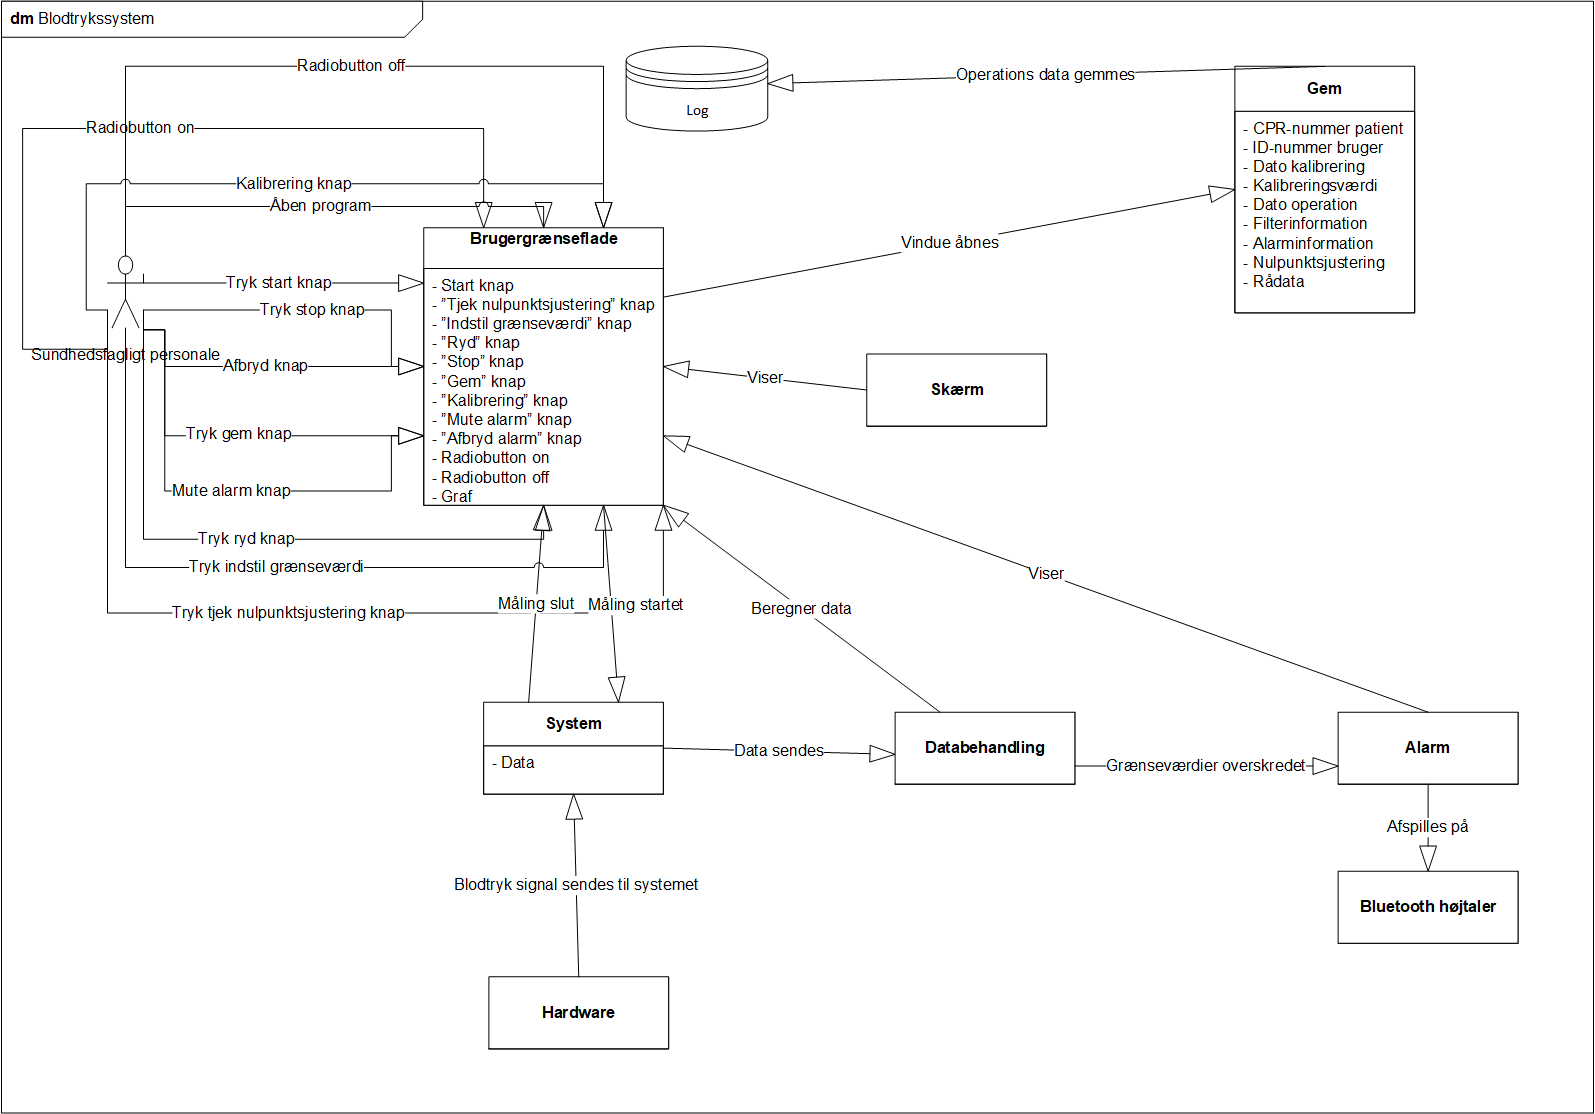
\includegraphics[width=1\linewidth]{Arkitektur_og_design/Softwarearkitektur/overordnetdomain}
	\label{fig:overordnetdomain}
	\caption{Overordnet domænemodel}
\end{figure}

Ovenstående figur \vref{fig:overordnetdomain} illustrerer den overordnede domænemodel, som viser både hardware og software. Domæneklassrne fandt vi efter en navneords analyse af vores fully dressed use cases, hvor vi fandt frem til brugergrænseflade, sundhedsfagligt personale, log, skærm, gem, system, databehandling, alarm og bluetooth højtaler.  Log domænet er en tekstfil, hvor oplysninger fra operationen gemmes i.

\subsection{Domænemodel for software}
  
Ud fra vores kendskab til domænet, har vi lavet en software-domænemodel, hvor vi får et overblik over, hvilke domæneklasser vores software skal indeholde. 

\clearpage

\begin{figure}[h!]
	\centering
	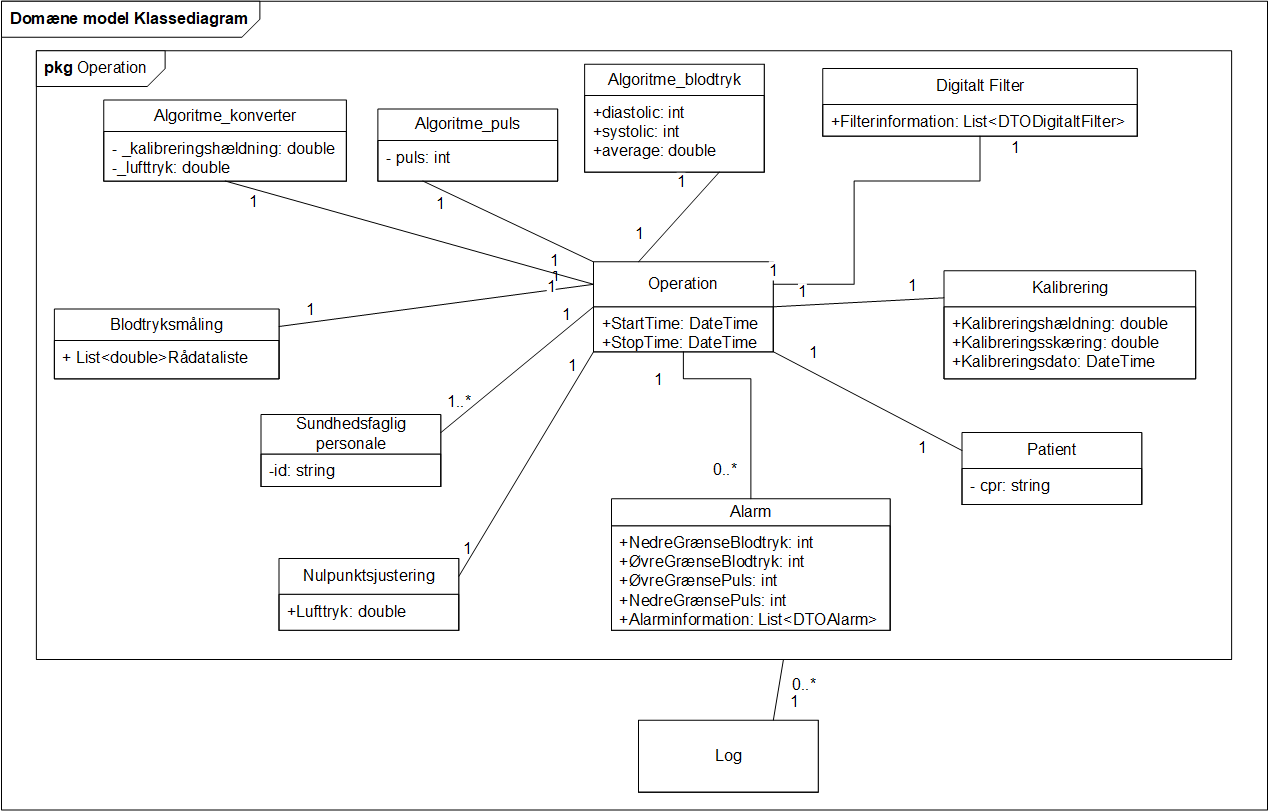
\includegraphics[width=1\linewidth]{Arkitektur_og_design/Softwarearkitektur/classdomain}
	\label{fig:classdomain}
	\caption{Domænemodel for software}
\end{figure}

Ovenstående figur \vref{fig:classdomain} viser systemets domæne for softwaren og hvilke klasser dette er bestående af.  Herudover viser den relationen mellem de forskellige domæneklasser og operationen. For eksempel kan der ved 1 operation være 0 til mange alarmer, som er illustreret ved "0..*". Modellen viser også en oversigt over klassernes tilhørende attributter og typerne af disse. Typerne har vi rationaliseret os frem til ved viden om at vores målinger vil være decimaltal (doubles), vores beregner vil vi gerne have vist i heltal (int), id og cpr er hensigtmæssigt at gemme som en string, og så vi nogle start- og stoptidspunkter som er oplagte at lave som DateTime. 

Ud fra vores use cases er vi kommet frem til, at ovenstående domæneklasser kan beskrive vores domæne tilstrækkeligt. Det gjorde vi, som tidligere nævnt, ved at lave en navnordsanalyse af vores fullydressed use cases. Ud fra denne fandt vi domæneklasserne: sundhedsfagligt personale, nulpunktsjustering, patient, alarm, kalibrering, digitalt filter, blodtryksmåling samt log. Ud fra disse gav det mening at samle det hele under klassen operation, som er vores brugssituation. Vi indså, at vi manglede klasser for vores databehandling. Dette delte vi op i tre klasser. En til pulsalgoritme, en til blodstryksalgoritme og en klasse til at konvertere fra volt til mmHg. 

Dernæst lavede vi et overordnet tomt klassediagram, som er udformet på baggrund af vores use cases. Klasserne fra software domænemodellen er en del af vores Model package, som indeholder domæneklasser og dtoklasser. 

\clearpage

\begin{figure}[h!]
	\centering
	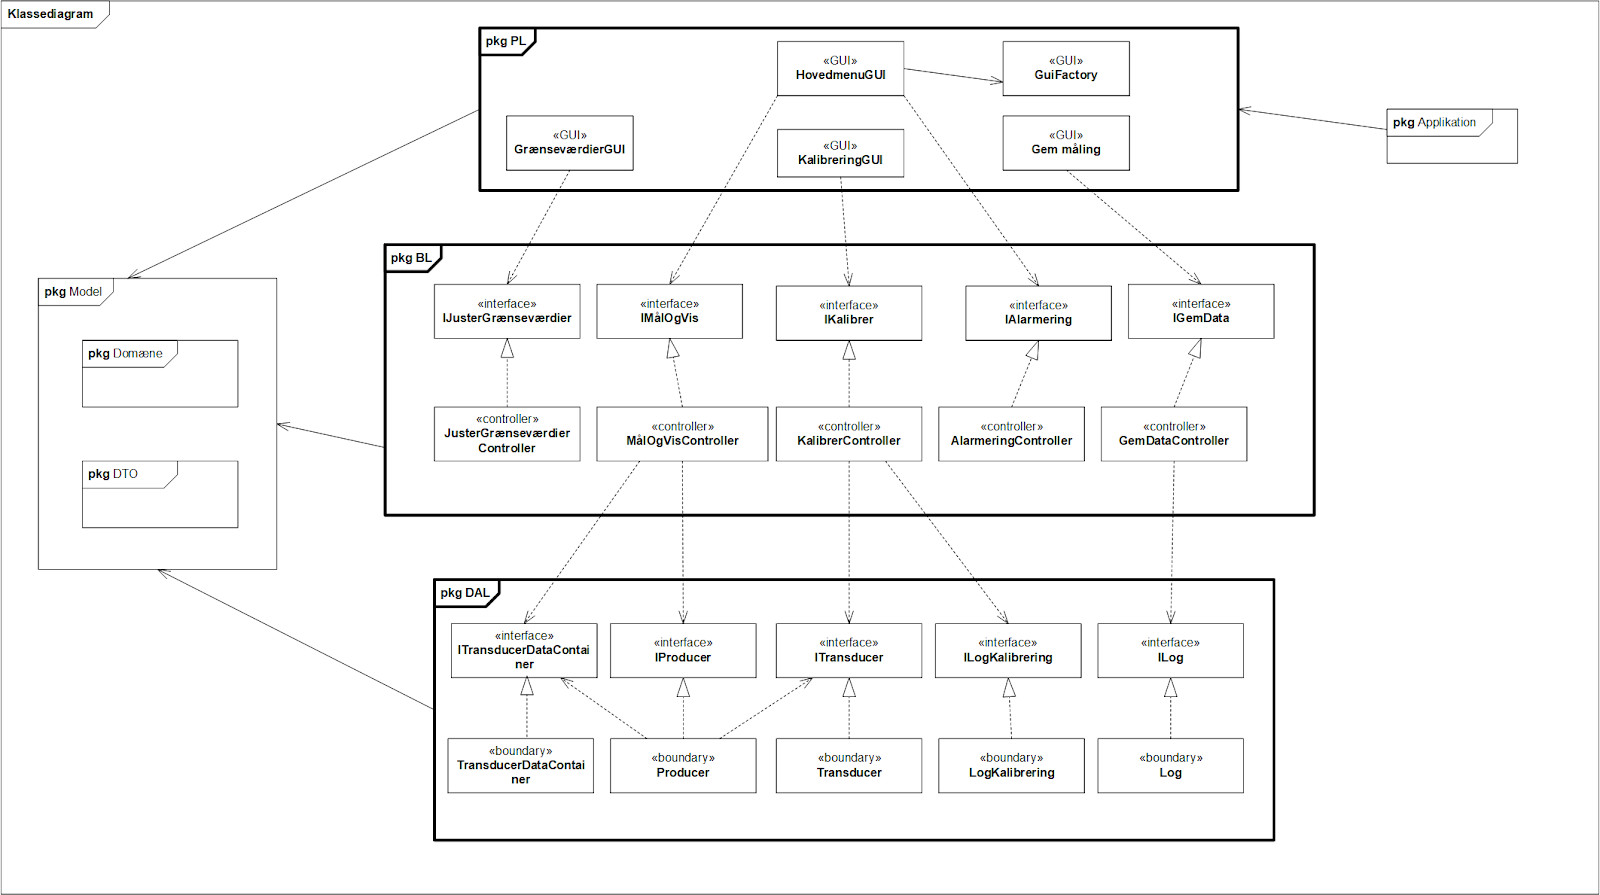
\includegraphics[width=1\linewidth]{Arkitektur_og_design/Softwarearkitektur/tomclass}
	\label{fig:tomclass}
	\caption{Klassediagram uden attributter og metoder}
\end{figure}

Klassediagrammet på figur \vref{fig:tomclass} viser opbygningen af softwaren. Vi har valgt at bygge vores system op efter trelagsmodellen, med præsentationslag (PL), businesslag (BL) og datalag (DAL). Dette er en god opbygning af et større system, som skal indhente, behandle og vise data.

\vspace{0.5 cm}
\input{Arkitektur_og_design/Design_Hardware/Design_hardware}
\input{Arkitektur_og_design/Design_Software/Design_software}



	\chapter{Implementering og test}

\section{Hardwareimplementering}
Alle dele af projektets hardware er blevet analyseret og designet og derefter implementeret. Vi startede med at udregne komponenter til forstærkeren, som vi på forhånd vidste hvordan skulle opbygges. Efter beregningerne kunne forstærkeren opbygges på fumlebræt. Efter at hver del er blevet implementeret på fumlebrættet er det blevet modultestet. På denne måde er vi sikre på, at hvert delelement af projektets hardware virker som forventet. På fumlebrættet er forstærkeren, subtractoren og Sallen-Key filteret derved implementeret og modultestet enkeltvis for at se om de gav de forventede værdier. Efterfølgende blev det hele sat sammen til et kredsløb og systemet kunne derefter integrationstestes. 

\begin{figure}[h!]
	\centering
	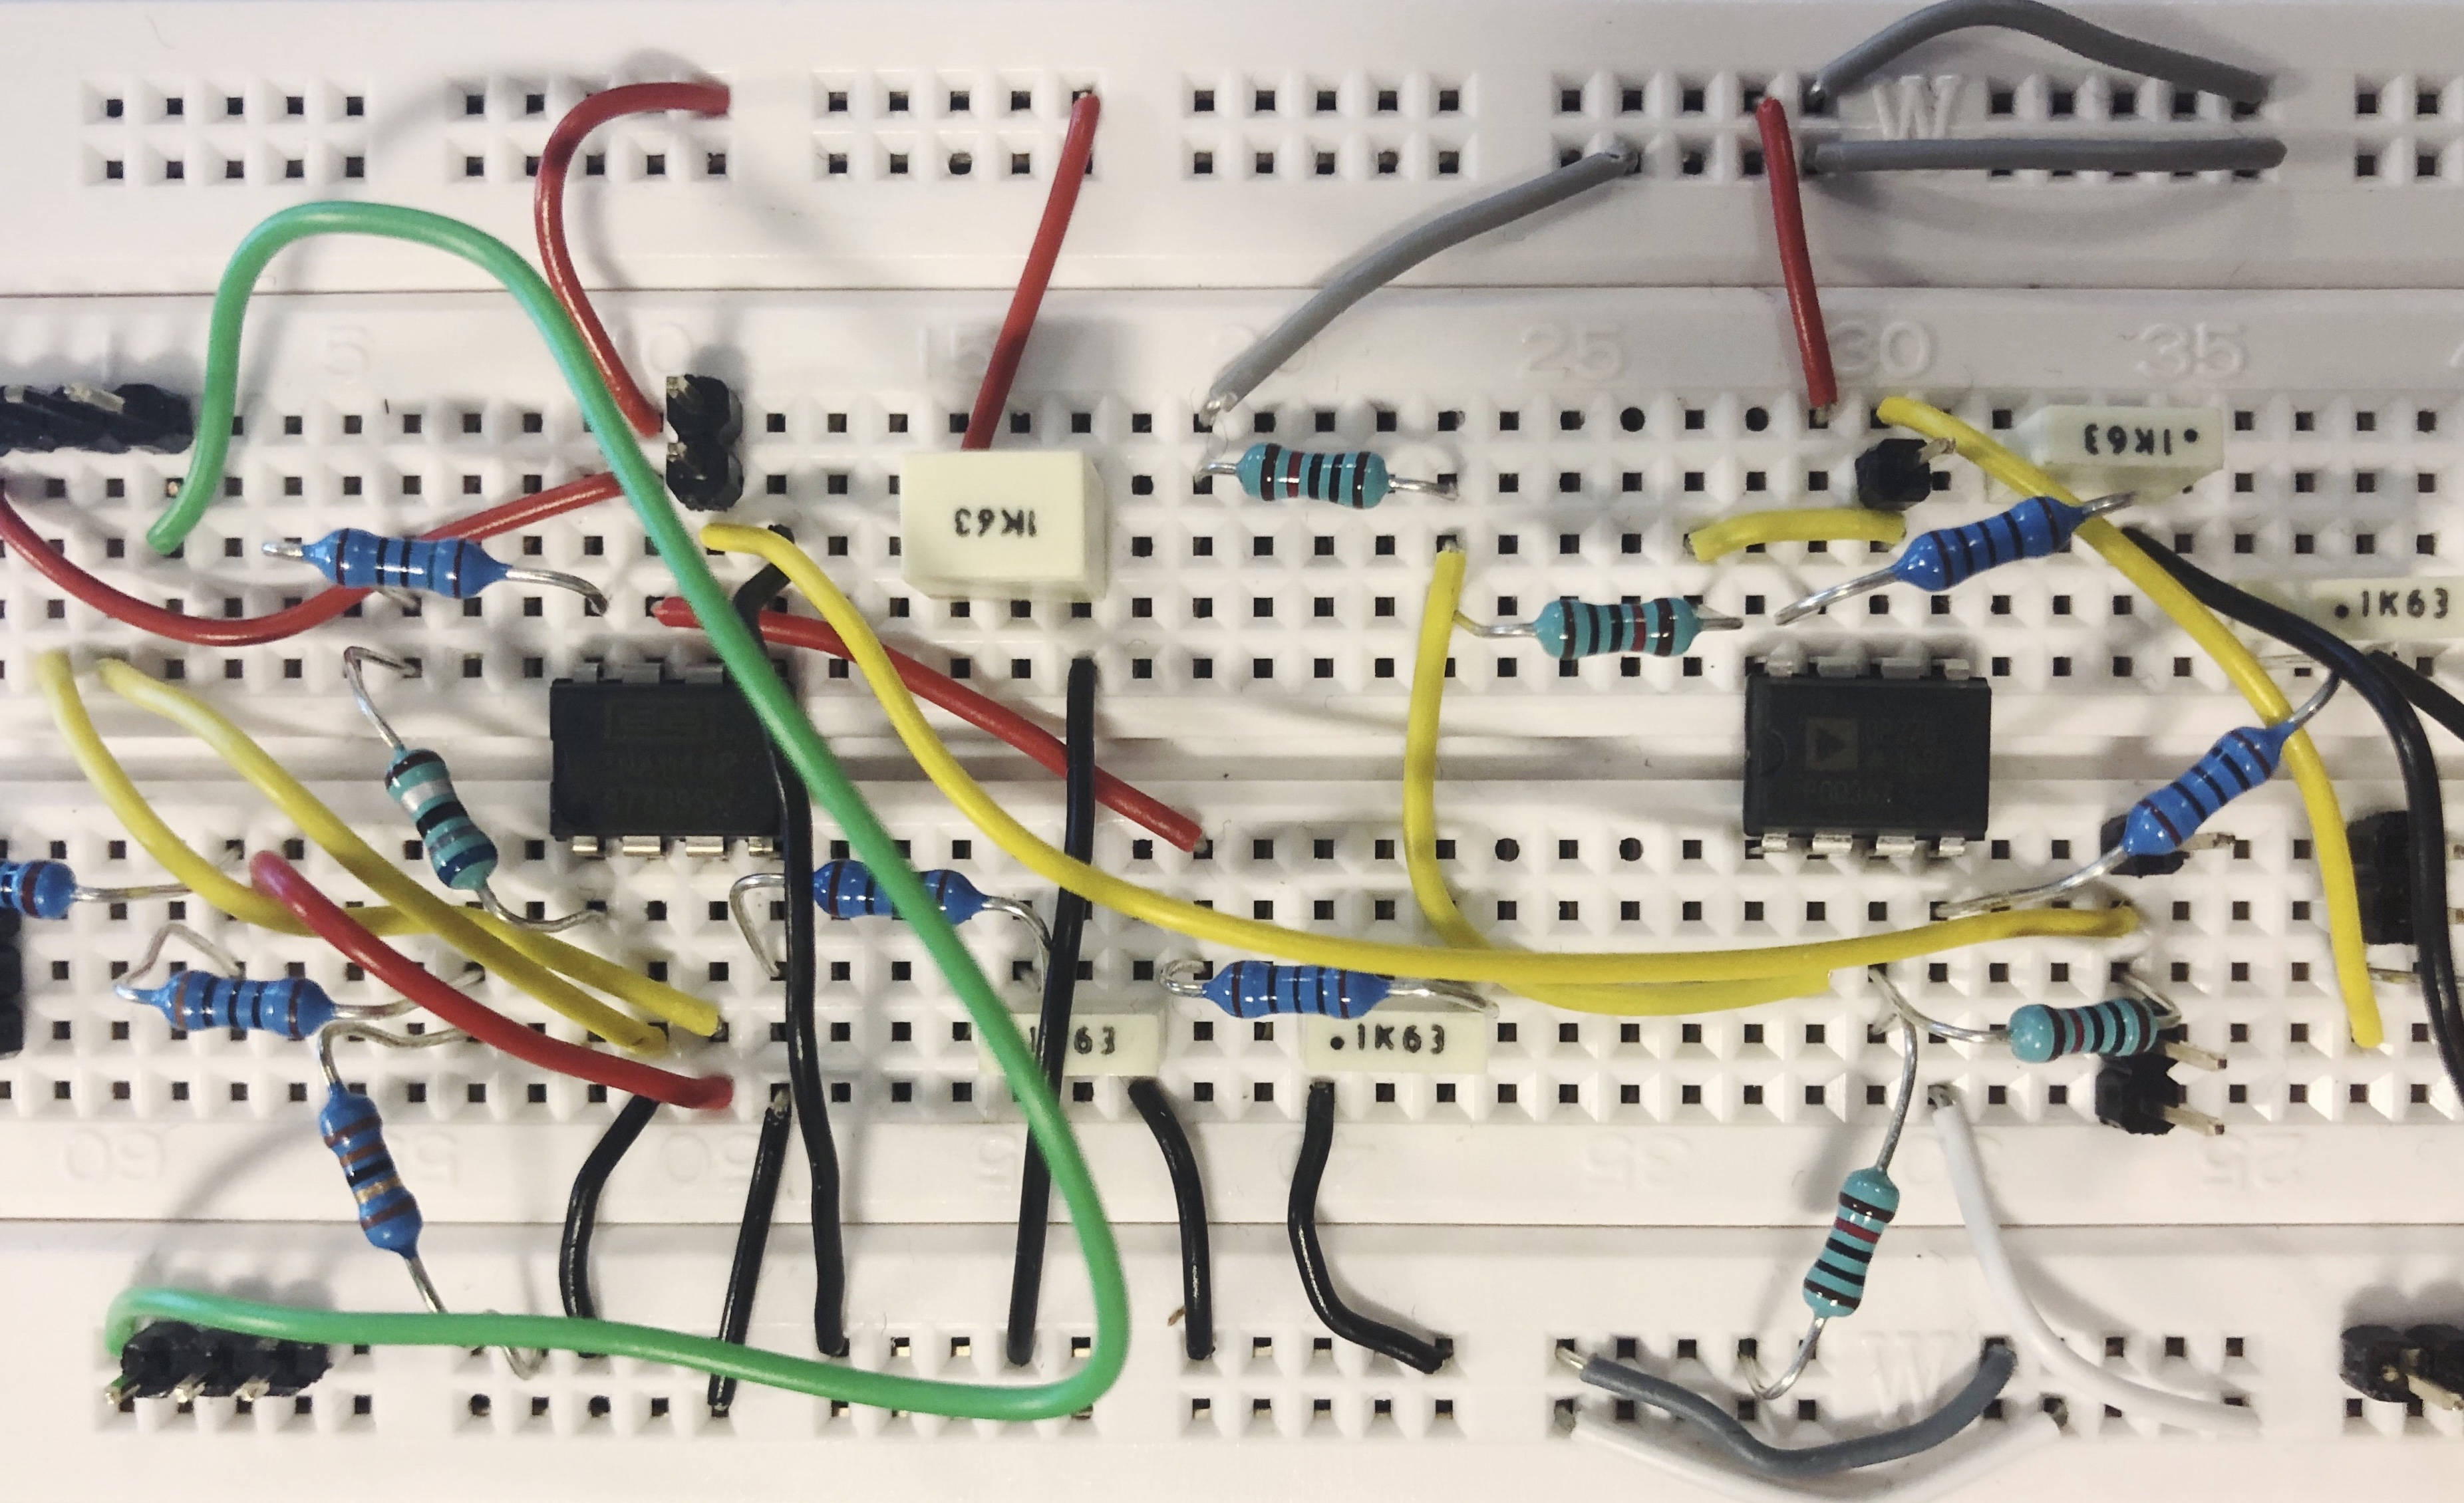
\includegraphics
	[width=0.54\linewidth]{../Rapport/Implementering_og_test/Hardware/forstaerkerogsubtractor2}
	\caption{Opbygning af forstærker(til venstre) og subtractor (til højre) på fumlebræt}
	\label{fig:forstaerkerogsubtractor1}
\end{figure}

\begin{figure}[h!]
	\centering
	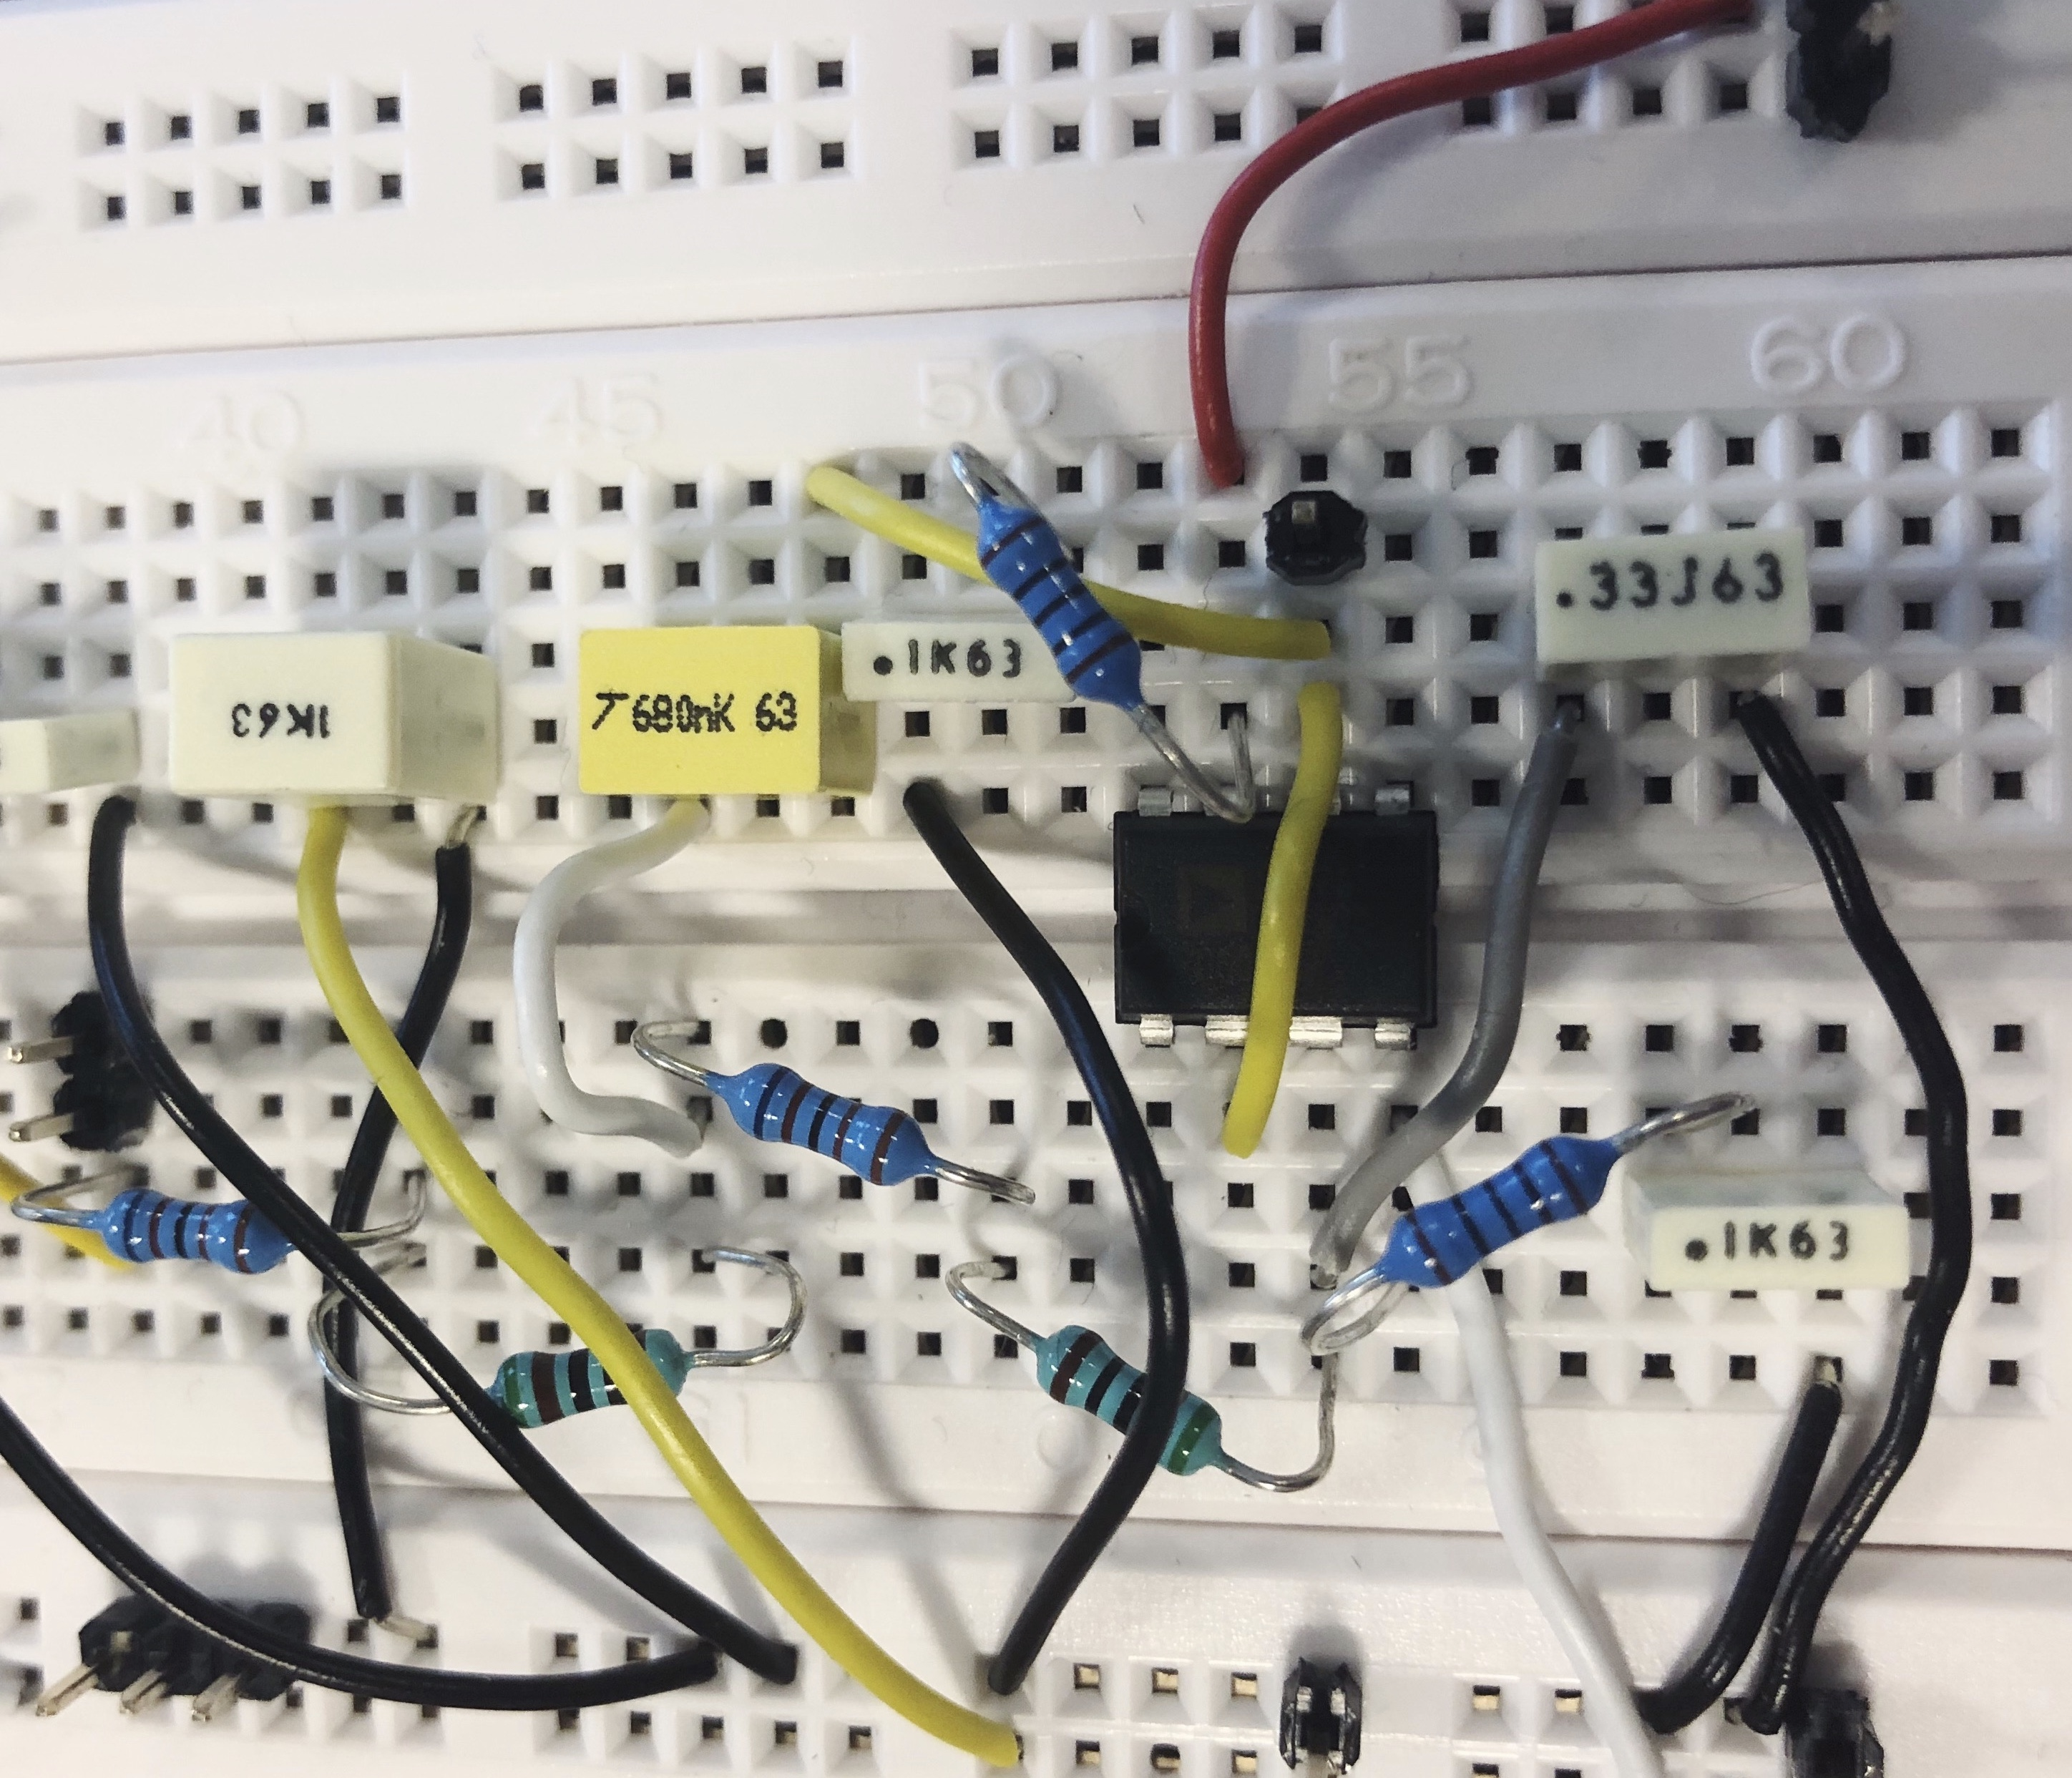
\includegraphics
	[width=0.54\linewidth]{../Rapport/Implementering_og_test/Hardware/filter2}
	\caption{Opbygning af filter på fumlebræt}
	\label{fig:filter1}
\end{figure}

Efter integrationstesten blev kredsløbet tegnet i Multisim. Det tegnede kredsløb i Multisim blev til slut overført til ultiboard, hvor de tilhørende komponenter blev placeret på printpladen. Printet blev testet og sendt til EuroCircuits. De beregnede komponenter i analyse-delen er til slut loddet på den færdige printplade og systemet blev testet en sidste gang. 

For kredsløbet i Multisim henvises til figur \vref{fig:Multisim2}. Nedenfor vises designet af printpladen i Ultiboard da det var klar til print samt printpladen, der er loddet med alle komponenter.

\begin{figure}[h!]
	\centering
	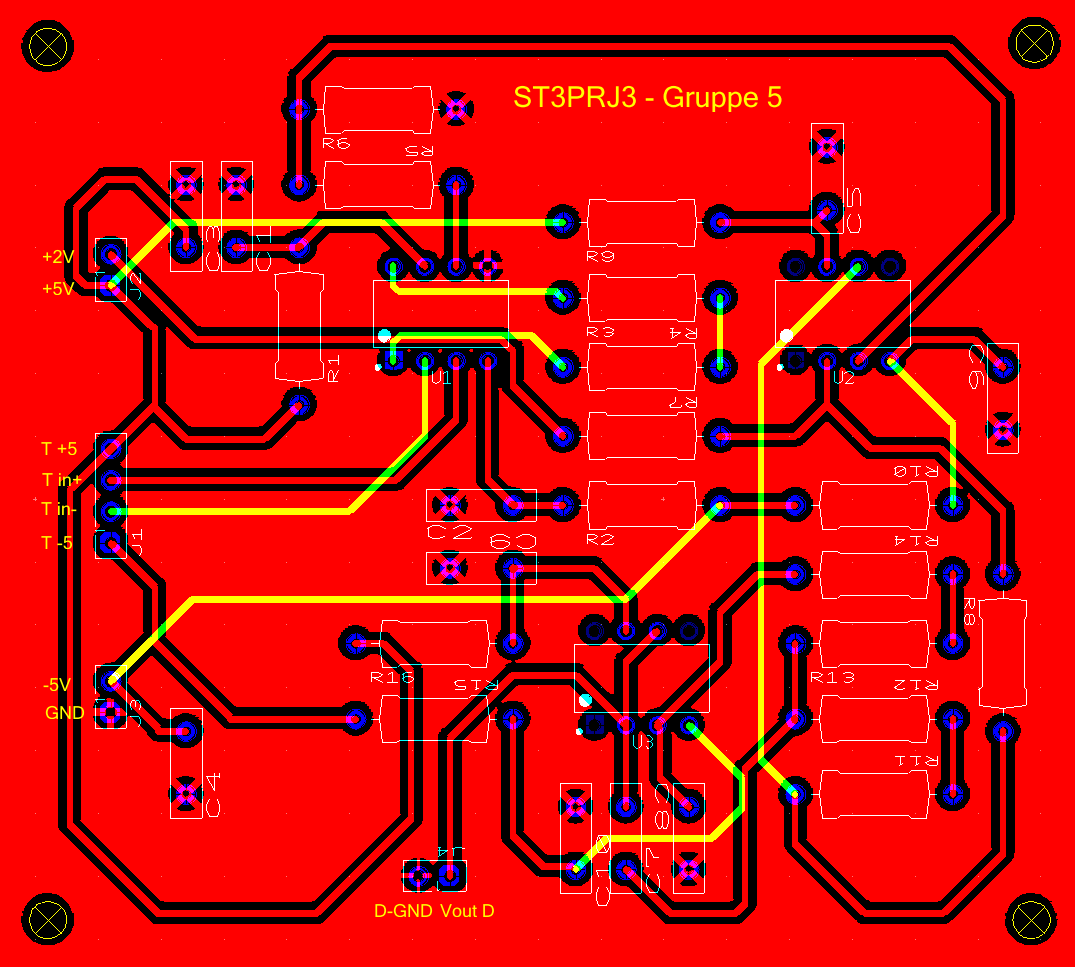
\includegraphics[width=0.5\linewidth]{../Rapport/Implementering_og_test/Hardware/Ultiboard}
	\caption{Print i Ultiboard}
	\label{fig:ultiboard1}
\end{figure}

\section{Softwareimplementering}
I implementeringsfasen startede gruppen ud med at lave et ”skelet” for programmeringen ud fra vores klassediagram, så det var opdelt og klar til at blive kodet efter 3 lags-modellen. Da vi blev klar til at gå i gang med at kode begav vi os til at uddelegere forskellige programmeringsopgaver. Hvert medlem startede med at påtage sig nogle små opgaver, som var nogle basale ting. Efter udførslen af små-opgaverne blev der uddelegeret use cases, som man fik ansvaret for, at var klar og funktionel til deadline. Uddelegeringen af opgaverne skete ved brug af arbejdsmetoden scrum, se afsnit - Herefter blev de forskellige use cases sat sammen, og testet på tværs af lagene ud fra programmets funktionalitet, der er defineret i kravspecifikationen. 

Hele vores system er skrev i programmeringssproget er C\# og er skrevet vha. programmerings programmet Visual Studios 2017.  Vi har gennem 1., 2. og 3. semester skrevet i sproget C\# i undervisningen, og derfor har det været oplagt at skrive i dette sprog. Alle i gruppen har endvidere downloadet programmet ”GitHub”, hvilket har gjort det muligt at alle gruppens medlemmer har kunne sidde og arbejde i det samme dokument. Dette har gjort programmeringsprocessen en hel del mere overskuelig idet vi får alle dele til at spille sammen med det samme, og ikke sætter det tilsammen til sidst, hvor der kan forkomme et store problemer.




\clearpage
\section{Test af hardware}
\subsection{Modultest}
Før at vi kunne teste det samlede system bestående af både hardware og software, måtte vi foretage nogle modultests af de enkelte dele i hardwaren. Forstærkeren, subtractoren samt antialiaseringsfilteret er blevet testet på fumlebrættet, og i forbindelse med disse test har vi skiftet mellem at bruge en spændingsdeler og en tryktransducer som var tilsluttet vandsøjlen. Da testene var godkendt, kunne vi tilkoble alt hardwaren og lave integrationstest.


\subsubsection{Forstærker}
I testen for forstærkeren brugte vi en spændingsdeler, da Analog Discovery ikke kan levere en lav nok spænding uden at være påvirket af støj. Spændingsdelerens skulle levere en lav spænding på 12,5 mV eller lavere, da transducerens output tilsvarende er en lav spænding. De 12,5 mV er beregnet under design afsnittet for forstærkeren. Spændingsdeleren fungerede derfor som en erstatning af transduceren, hvor vi blot selv kunne bestemme hvilket type signal vi ville sende igennem forstærkeren.

\textbf{Test med spændningsdeler}

For at teste om signalet blev forstærket 320 gange af forstærkeren, sendte vi 4 V gennem spændingsdeleren og forstærkeren, og målte på udgangen af forstærkeren. Spændingsdeleren var i denne test designet til at kunne levere et output svarende til 320 gange mindre end 4 V, hvilket svarer til 12,5 mV, som er transducerens max output. Denne viden kunne vi benytte, så inputtet til spændingsdeleren og outputtet fra forstærkeren burde være det samme.

Da vi målte på udgangen af forstærkeren, fik vi et en spænding på 4 V, hvilket stemte overens med vores forventede resultater.


\textbf{Test med transducer og vandsøjle}

I denne test erstattede vi spændingsdeleren med transduceren, som blev tilsluttet vandsøjlen. Der blev udført en række tests med forskellige tryk på transduceren, for at undersøge om signalet blev forstærket op 320 gange, samt teste lineariteten og nøjagtigheden af vores målinger.

Nedenstående graf repræsenterer testresultaterne fra et tryk på 0, 10, 50 og 100 mmHg.


\vspace{0.5 cm}

\begin{figure}[h!]
	\centering
	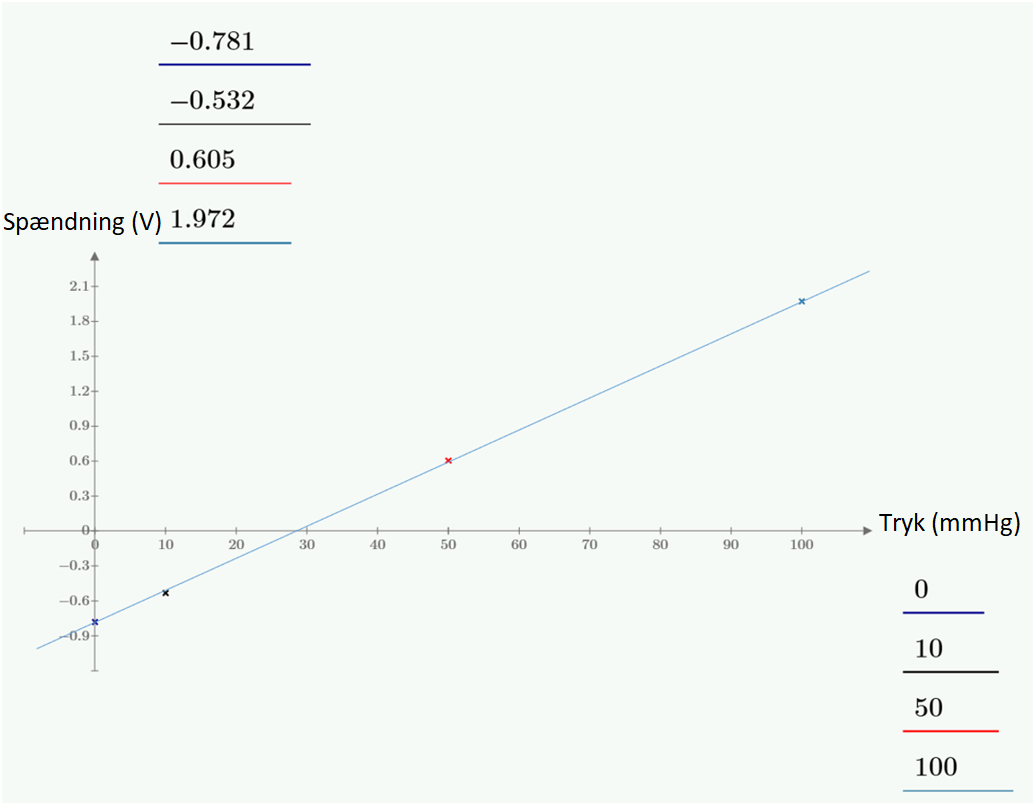
\includegraphics[width=0.6\linewidth]{../Rapport/Implementering_og_test/Hardware/forstaerker}
	\caption{Spænding som funktion af tryk}
	\label{fig:forstaerker}
\end{figure}

\clearpage

På x-aksen er tryk i mmHg, og på y-asken er spænding i V. Det ses at der er en god lineær sammenhæng mellem tryk og spænding, samt at signalet er blevet forstærket. Da vi på vandsøjlen kun kan måle op til 100 mmHg antager vi at denne sammenhæng fortsætter, og kan opstille følgende regnestykke: 

\[\frac{250 mmHg}{100 mmHg} = 2,5 \]
\[ 1,972 V \cdot 2,5 = 4,93 V \]
\[ 4,93 V - 0,781 V = 4,149 V \]

Ovenstående værdier kommer fra figur \textbf{X}, hvor de 1,972 V er spændingen ved 100 mmHg. De 4,93 V er den forventede spænding ved 250 mmHg, hvor det atmosfæriske tryk er inkluderet. For at finde den korrekte værdi for 250 mmHg uden atmosfærisk tryk trækkes de 0,781 V fra, hvilket er skæringen med y-aksen, som på denne graf er tilsvarende det atmosfæriske tryk. Da vores antagelser ligger udenfor det målbare område er det regnestykket ekstrapolært, og er dermed forbundet med en større usikkerhed.

Ud fra tidligere beregninger vil vi forvente at et tryk på 250 mmHg vil have en spænding på 4 V, hvilket stemmer godt overens med vores test. De specifikke måleresultater findes i bilag for test af hardwaren.

\subsubsection{Subtractor}

For at teste subtractoren brugte vi waveforms til at genere to signaler. Et DC-signal på 2 V, hvilket subtractoren bruger til at trække et signal ned med 2 V. Det andet signal var et sinussignal, som blev sendt gennem subtractoren. I testen forventede vi, at subtractoren ville sænke sinussignalet 2 V ned i dens amplitude. Vi sendte et sinussignal ind med et offset på 2 V, for at hæve signalet, som vi derefter vha. subtractoren kunne sænke. Vi målte signalerne ved brug af waveforms scope funktion.

\begin{figure}[h!]
	\centering
	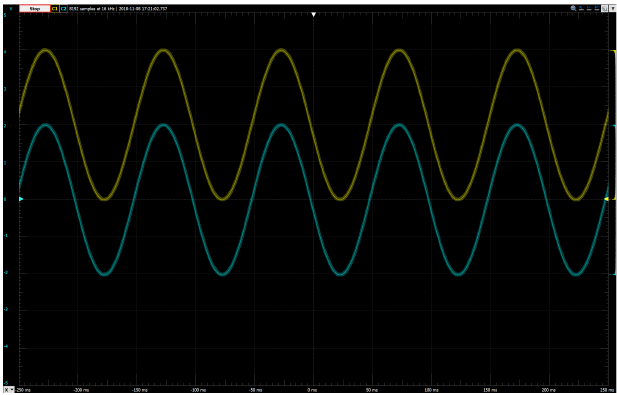
\includegraphics[width=0.72\linewidth]{../Rapport/Implementering_og_test/Hardware/subtractor}
	\caption{Test af subtractor. På y-aksen ses spændning (V), og på x-aksen ses tid (sekunder)}
	\label{fig:subtractor}
\end{figure}

På ovenstående screenshot ses den gule kurve, som et sinussignal med en amplitude på 2 V og et offset på 2 V. Der benyttes et sinussignal, for at teste subtractorens nedeskalering af forskellige amplituder. Den blå kurve er outputtet fra subtractoren, hvilket har sænket det oprindelige sinussignal med 2 V.

Subtractoren virkede derfor som den skulle, i og med at den kunne sænke signalet med de ønskede 2 V.


\subsubsection{Filter}

Da vi testede filteret, sendte vi et sinussignal ind på filteret med en amplitude på 2 V. For at undersøge filtrets dæmpning gav vi signalet 24 forskellige hertz i et range på 10 til 500 Hz. Resultaterne er påvist på nedenstående bodeplot.

\begin{figure}[h!]
	\centering
	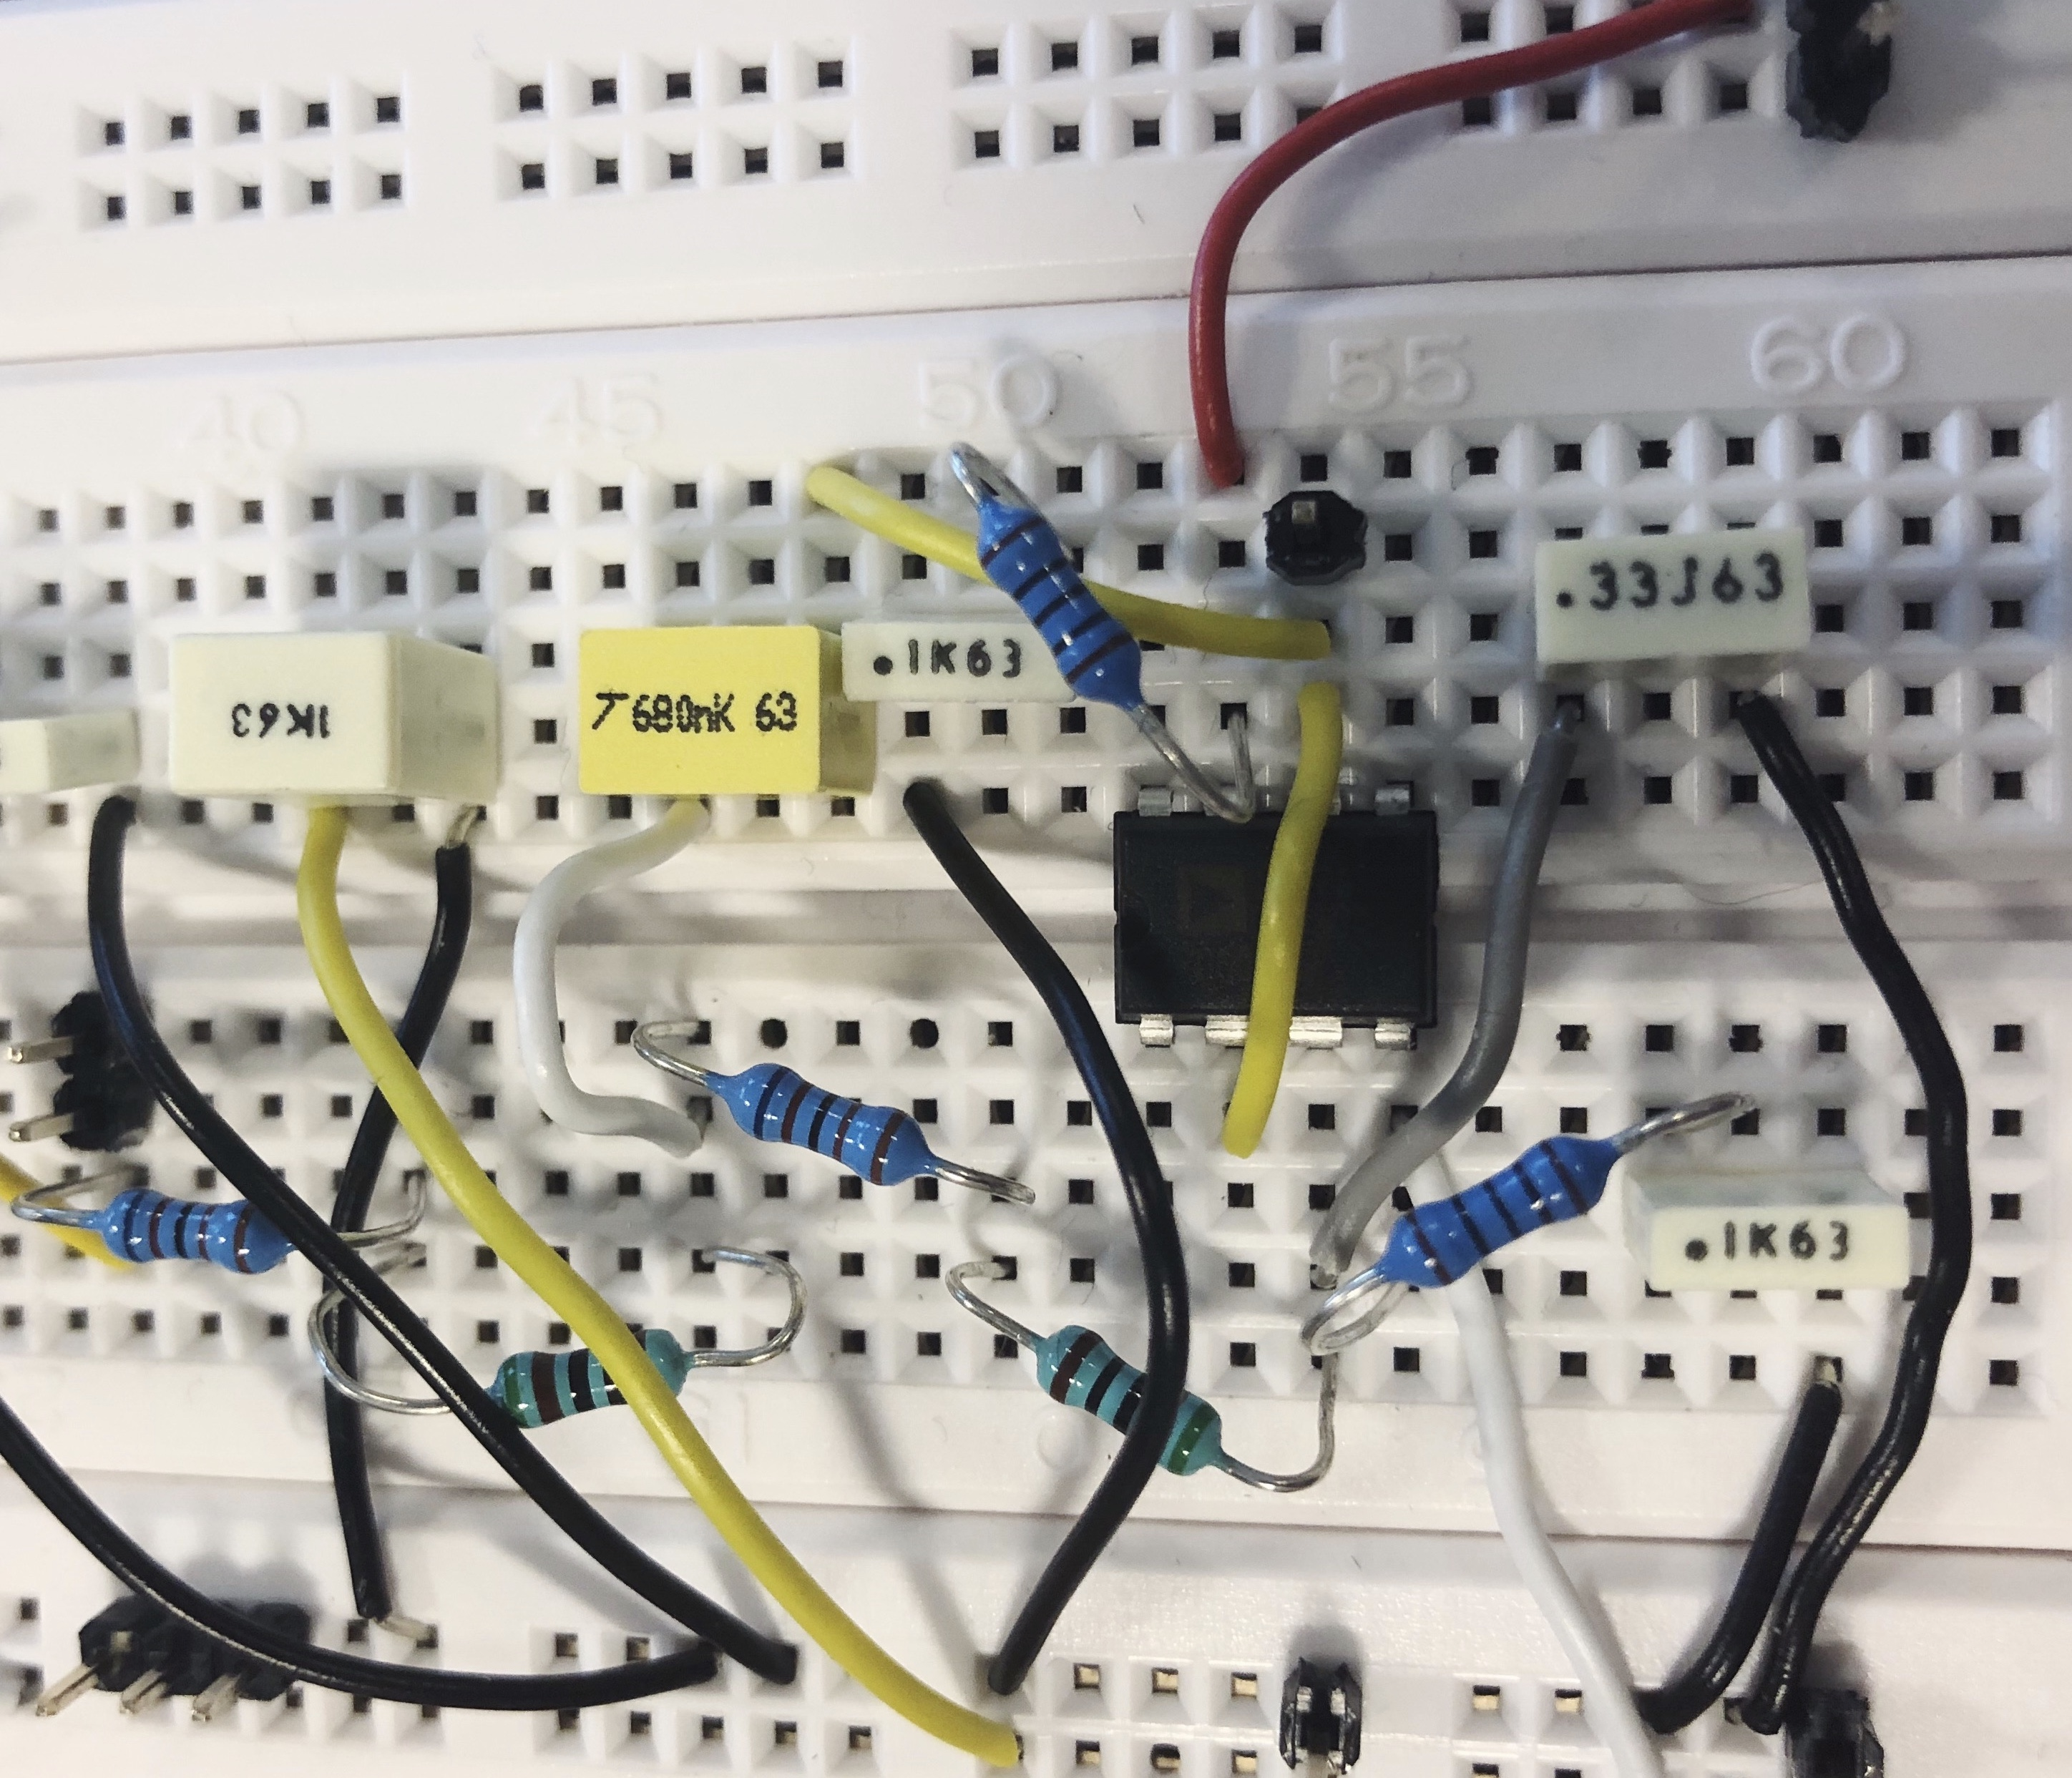
\includegraphics[width=0.8\linewidth]{../Rapport/Implementering_og_test/Hardware/filter2}
	\caption{Bodeplot af 2. ordens antialiaseringsfilteret}
	\label{fig:filter}
\end{figure}

Knækfrekvensen er påtegnet som den sorte vertikale linje på figur X, hvilket er det fjerde målepunkt på grafen, som er 50 Hz. Filteret har allerede ved 50 Hz har sænket signalet med -3 dB, hvilket skyldes at filterets dæmpningsfaktor er 0,707, som giver det fladeste bodeplot. Tager man 20*log(0,707) fås der tilsvarende en værdi på -3 dB.

Det ses at signalet dæmper 40 dB pr dekade, hvilket stemmer overens med vores ventede resultat. De specifikke måleværdier kan findes i bilag for test af hardwaren.

Kravet er at filteret skal dæmpe 20 dB over den dekade der er til rådighed, så i teorien har vi ikke brug for et 2. ordensfilter. Dog i tilfælde af at vi brugte 1. ordensfilter, skulle alt performe fuldstændigt perfekt, hvilket var en risiko vi ikke var villige at tage, og derfor benytter vi et 2. ordensfilter.

\clearpage

\subsubsection{Integrationstest med vandsøjle}

Da modulttestene var gennemført med tilfredsstillelse, blev hele systemet sammenkoblet, således der kunne laves en integrationstest for hele systemet. Formålet med denne test er at undersøge, om hele systemet kan integrere fornuftigt med hinanden, samt undersøge hvilke output de forskellige tryk på vandsøjlen giver, og dermed finde en sammenhæng mellem tryk og spænding.
Der blev testet ved 5 forskellige tryk, hvilke var 0, 10, 25, 50, 75 og 100 mmHg. Vi forventede at få en talrække indenfor -2 V og 2 V, da forstærkeren burde forstærke op i et spænd fra 0-4 V, og subtractoren herefter ville sænke signalet med 2 V.

Resultaterene fra testen er blevet plottet på nedenstående figur:

\begin{figure}[h!]
	\centering
	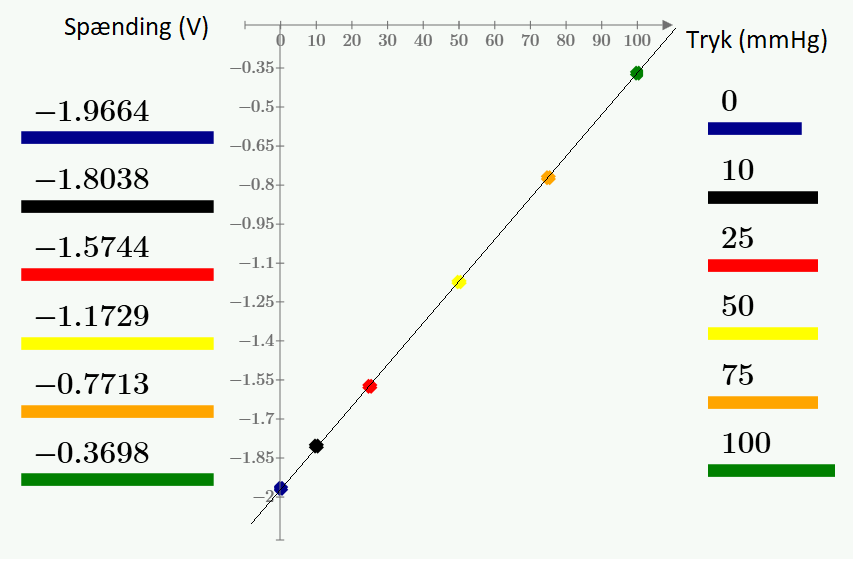
\includegraphics[width=0.8\linewidth]{../Rapport/Implementering_og_test/Hardware/integrationsplothw}
	\caption{Spænding som funktion af tryk}
	\label{fig:integrationsplot}
\end{figure}

Det ses at punkterne ligger for en lige linje, og der er derfor en god sammenhæng mellem tryk og spænding. Derudover ligger værdierne indenfor det forventede område, hvilke er -2 og 2 V, og testen gik derfor som forventet.


Ovenstående tests gav os en god indikation for, at hardwaren var velfungerende, og var klar til at blive realiseret i multisim.

\clearpage
\section{Test af software}
\subsection{Modultest}
\subsection{Integrationstest}
	\chapter{Resultater}
\section{Hardwareresultater}
\section{Diskussion af resultater}
\section{Reresultater}

Ud fra vores accepttest blev alle vores krav testet. Resultaterne giver et billede over hvilke funktioner som virkede optimalt, og hvilke der ikke gjorde. 

\begin{table}[h!]
	\centering
	\begin{tabular}{llllll}
		\multicolumn{6}{l}{\cellcolor[HTML]{187ABD}\textbf{Resultater for accepttest af Use Case 1: Mål og vis blodtryk og puls}} \\ \hline
		\textbf{Use Case 1: Mål og} & \multicolumn{1}{l|}{} &  & \multicolumn{1}{l|}{} & \textbf{Ext. 1: Digitalt filter} &  \\
		\textbf{vis blodtryk og puls} & \multicolumn{1}{l|}{} &  & \multicolumn{1}{l|}{} & \textbf{vælges fra} &  \\ \cline{1-2} \cline{5-6} 
		\textbf{Test} & \multicolumn{1}{l|}{\textbf{Resultat}} &  & \multicolumn{1}{l|}{} & \textbf{Test} & \textbf{Resultat} \\ \cline{1-2} \cline{5-6} 
		1.1 & \multicolumn{1}{l|}{OK} &  & \multicolumn{1}{l|}{} & 1.2.1 & OK \\ \cline{1-2} \cline{5-6} 
		1.2 & \multicolumn{1}{l|}{OK} &  & \multicolumn{1}{l|}{} &  &  \\ \cline{1-2} \cline{5-6} 
		1.3 & \multicolumn{1}{l|}{OK} &  & \multicolumn{1}{l|}{} &  &  \\ \cline{1-2} \cline{5-6} 
		1.4 & \multicolumn{1}{l|}{OK} &  & \multicolumn{1}{l|}{} &  & 
	\end{tabular}
\end{table}

\begin{table}[h!]
	\centering
	\begin{tabular}{llllll}
		\multicolumn{6}{l}{\cellcolor[HTML]{187ABD}\textbf{Resultater for accepttest af Use Case 2: Juster grænseværdier}} \\ \hline
		\textbf{Use Case 2: Juster} & \multicolumn{1}{l|}{} &  & \multicolumn{1}{l|}{} & \textbf{Ext. 2a: Systemet} &  \\
		\textbf{grænseværdier} & \multicolumn{1}{l|}{} &  & \multicolumn{1}{l|}{} & \textbf{afviser justering} &  \\ \cline{1-2} \cline{5-6} 
		\textbf{Test} & \multicolumn{1}{l|}{\textbf{Resultat}} &  & \multicolumn{1}{l|}{} & \textbf{Test} & \textbf{Resultat} \\ \cline{1-2} \cline{5-6} 
		2.1 & \multicolumn{1}{l|}{OK} &  & \multicolumn{1}{l|}{} & 2.1.1 & OK \\ \cline{1-2} \cline{5-6} 
		2.2 & \multicolumn{1}{l|}{OK} &  & \multicolumn{1}{l|}{} & 2.1.2 & FAIL \\ \cline{1-2} \cline{5-6} 
		2.3 & \multicolumn{1}{l|}{OK} &  & \multicolumn{1}{l|}{} & 2.1.3 & OK \\ \cline{1-2} \cline{5-6} 
		2.4 & \multicolumn{1}{l|}{OK} &  & \multicolumn{1}{l|}{} & 2.1.4 & Ikke testet
	\end{tabular}
\end{table}

\begin{table}[h!]
	\centering
	\begin{tabular}{llllll}
		\multicolumn{6}{l}{\cellcolor[HTML]{187ABD}\textbf{Resultater for accepttest af Use Case 3: Alarmering}} \\ \hline
		\textbf{Use Case 3:} & \multicolumn{1}{l|}{} &  & \multicolumn{1}{l|}{} & \textbf{Ext. 3a: Sundheds-} &  \\
		\textbf{Alarmering} & \multicolumn{1}{l|}{} &  & \multicolumn{1}{l|}{} & \textbf{fagligt personale} &  \\
		& \multicolumn{1}{l|}{} &  & \multicolumn{1}{l|}{} & \textbf{muter alarmen} &  \\ \cline{1-2} \cline{5-6} 
		\textbf{Test} & \multicolumn{1}{l|}{\textbf{Resultat}} &  & \multicolumn{1}{l|}{} & \textbf{Test} & \textbf{Resultat} \\ \cline{1-2} \cline{5-6} 
		(Hovedscenarie testet & \multicolumn{1}{l|}{} &  & \multicolumn{1}{l|}{} & 3.1.1 & OK \\ \cline{5-6} 
		gennem andre Use & \multicolumn{1}{l|}{} &  & \multicolumn{1}{l|}{} & 3.1.2 & OK \\ \cline{5-6} 
		Cases) & \multicolumn{1}{l|}{} &  & \multicolumn{1}{l|}{} & 3.1.3 & OK
	\end{tabular}
\end{table}

\begin{table}[h!]
	\centering
	\begin{tabular}{llllll}
		\multicolumn{6}{l}{\cellcolor[HTML]{187ABD}\textbf{Resultater for accepttest af Use Case 4: Gem data}} \\ \hline
		\textbf{Use Case 4: Gem} & \multicolumn{1}{l|}{} &  & \multicolumn{1}{l|}{} & \textbf{Ext. 4a: Data ikke} &  \\
		\textbf{data} & \multicolumn{1}{l|}{} &  & \multicolumn{1}{l|}{} & \textbf{gemt} &  \\ \cline{1-2} \cline{5-6} 
		\textbf{Test} & \multicolumn{1}{l|}{\textbf{Resultat}} &  & \multicolumn{1}{l|}{} & \textbf{Test} & \textbf{Resultat} \\ \cline{1-2} \cline{5-6} 
		4.1 & \multicolumn{1}{l|}{OK} &  & \multicolumn{1}{l|}{} & 4.1.1 & FAIL \\ \cline{1-2} \cline{5-6} 
		4.2 & \multicolumn{1}{l|}{FAIL} &  & \multicolumn{1}{l|}{} & 4.1.2 & FAIL \\ \cline{1-2} \cline{5-6} 
		4.3 & \multicolumn{1}{l|}{FAIL} &  & \multicolumn{1}{l|}{} &  &  \\ \cline{1-2} \cline{5-6} 
		4.4 & \multicolumn{1}{l|}{FAIL} &  & \multicolumn{1}{l|}{} &  & 
	\end{tabular}
\end{table}

\clearpage

\begin{table}[h!]
	\centering
	\begin{tabular}{ll}
		\multicolumn{2}{l}{\cellcolor[HTML]{187ABD}\textbf{Resultater for accepttest af Use Case 4: Kalibrering}} \\ \hline
		\multicolumn{1}{l|}{\textbf{Use Case 4: Kalibrering}} &  \\ \hline
		\multicolumn{1}{l|}{\textbf{Test}} & \textbf{Resultat} \\ \hline
		\multicolumn{1}{l|}{5.1} & OK \\ \hline
		\multicolumn{1}{l|}{5.2} & OK \\ \hline
		\multicolumn{1}{l|}{5.3} & FAIL \\ \hline
		\multicolumn{1}{l|}{5.4} & FAIL
	\end{tabular}
\end{table}

Ud over de ovenstående tests af funktionelle krav er der også blevet lavet acceptests af de ikke-funktionelle krav. Resultaterne på testen ses her: 

\begin{table}[h!]
	\centering
	\begin{tabular}{lll}
		\multicolumn{3}{l}{\cellcolor[HTML]{187ABD}\textbf{Resultater for ikke-funktionelle krav}} \\ \hline
		\multicolumn{1}{l|}{\textbf{Krav nr.}} & \multicolumn{1}{l|}{\textbf{Krav}} & \textbf{Vurdering} \\
		\multicolumn{1}{l|}{} & \multicolumn{1}{l|}{} & \textbf{(OK/FAIL)} \\ \hline
		\multicolumn{1}{l|}{1} & \multicolumn{1}{l|}{Den skærm der benyttes af operatøren} & OK \\
		\multicolumn{1}{l|}{} & \multicolumn{1}{l|}{er den skærm, hvor man kan interagere} &  \\
		\multicolumn{1}{l|}{} & \multicolumn{1}{l|}{med systemet} &  \\ \hline
		\multicolumn{1}{l|}{2} & \multicolumn{1}{l|}{Den skærm, der benyttes af observatøren} & Ikke testet \\
		\multicolumn{1}{l|}{} & \multicolumn{1}{l|}{er den skærm, hvor man observerer grafen} &  \\
		\multicolumn{1}{l|}{} & \multicolumn{1}{l|}{samt værdier for systolisk-, diastolisk-, middel-} &  \\
		\multicolumn{1}{l|}{} & \multicolumn{1}{l|}{blodtryk og puls.} &  \\ \hline
		\multicolumn{1}{l|}{3} & \multicolumn{1}{l|}{Systemets GUI skal indeholde elementerne} & OK \\
		\multicolumn{1}{l|}{} & \multicolumn{1}{l|}{beskrevet under systembeskrivelsen i dokumentet} &  \\
		\multicolumn{1}{l|}{} & \multicolumn{1}{l|}{"Kravspecifikation" som findes i bilaget} &  \\ \hline
		\multicolumn{1}{l|}{4} & \multicolumn{1}{l|}{Systemets GUI skal kunne vise en graf inden for} & OK \\
		\multicolumn{1}{l|}{} & \multicolumn{1}{l|}{5 sekunder} &  \\ \hline
		\multicolumn{1}{l|}{5} & \multicolumn{1}{l|}{Systemet skal kunne stoppe målingen inden for} & OK \\
		\multicolumn{1}{l|}{} & \multicolumn{1}{l|}{5 sekunder} &  \\ \hline
		\multicolumn{1}{l|}{6} & \multicolumn{1}{l|}{Grafen samt de viste værdier skal kunne læses på} & OK \\
		\multicolumn{1}{l|}{} & \multicolumn{1}{l|}{op til 0,5 meters afstand. Farverne skal kunne skelnes} &  \\
		\multicolumn{1}{l|}{} & \multicolumn{1}{l|}{af personer med farveblindhed} & 
	\end{tabular}
\end{table}

Gruppen fik lov til at komme ud på Skejby sygehus og afprøve blodtryksmåleren på en gris. Forsøget gik ikke helt som forventet. Vi havde forventet nogle større udsving og har efterfølgende fundet ud af, at filteret havde to forkerte modstande på printpladen. Dette var skyld i en for hård filtrering af signalet og er efterfølgende blevet ændret.

\vspace{0.5 cm}
\begin{figure}[h!]
	\centering
	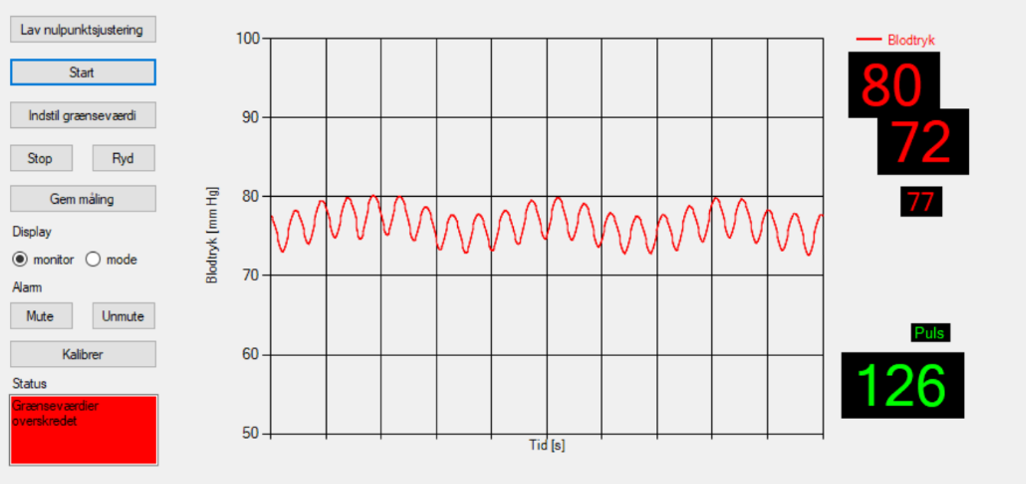
\includegraphics[width=0.7\linewidth]{Resultater/Resultater/gris}
	\label{fig:gris}
	\caption{Målt blodtryk på gris}
\end{figure}

\section{Diskussion af resultater}

Accepttesten gik udmærket, og vi fik valideret vores krav. Accepttesen bestod af 5 Use Cases, hvor hver Use Case indeholdt flere krav, der skulle testes. De fleste af kravene blev imødekommet, dog var der også flere som ikke gjorde. Kravene der ikke blev imødekommet skyldtes prioritering af forskellige arbejdsopgaver, hvor det var blevet nødvendigt at lægge arbejdsindsatsen ind på, at få alle ”Must have” kravene opfyldt, som det første.
Den første Use Case med ”Mål og vis blodtryk og puls” gik efter planen, og opfyldte alle de stillede krav. I denne Use Case var det de mest grundlæggende dele af vores system, som blev testet og var derfor prioriteret højt ift. at skulle bestå alle testene. Det lykkedes os at få foretaget en nulpunktsjustering samt at få vist blodtryk og puls på en graf via brugergrænsefladen, hvor grafen både kunne vises med digitalt filter og uden. 

Use Case 2 ”Justering af grænseværdier” gik som vi havde forventet. Det lykkedes os at kunne justere forskellige grænseværdier, hvor der kom en fejlmeddelelse, hvis grænserne virkede usandsynlige høje/lave.  En overskridning af grænseværdierne viste sig også fint i ”statusboksen”, som blinkede rødt og gav en alarmeringsbesked. Det lykkedes os dog ikke at få udført en ændring af grænseværdierne mens vi fik et signal ind, da testen ikke kunne udføres med signalet fra væskesøjlen. Væskesøjlen giver en puls på 0, og vil derfor gøre det umuligt for os at teste på, da der ikke kan justeres på pulsen. I stedet skulle der have været brugt en analog discovery til at sende et signal ind.

Use Case 3 ” Alarmering” blev testet parallelt med andre use cases idet de aktiverede alarmerne i forskellige sammenhænge. Vi valgte derfor ikke at lave nogle specifikke test af alarmen, udover hvor alarmen mutes. Når alarmen var i gang auditivt spillede tonerne c e g – g C, hvilket var det vi havde forventet. Samtidigt blinkede ”statusboksen” med en hertz på 2, og en duty cycle på 50%. 

Det lykkedes os desværre ikke at gemme vores data, som planlagt i Use Case 4 ”Gem data”. Efter at have gået vores kode for ”gem data” grundigt igennem står det nu klart for os, hvorfor data’en ikke bliver gemt. I koden bliver der oprettet nye instanser af hver klasse, hver gang der skal gemmes noget data. Dette medfører at data’en fra den klasse, som der gerne skulle gemmes fra ikke bliver overført til klassen, hvor vi gerne vil gemme det. Resultatet af det er at vi ikke får gemt noget data.
Udover at have oprettet flere instanser af klasserne opstod der også problemer under serialisering af den gemte data. 

Under testning af kalibreringen fandt vi ud af at vores system kalibrer korrekt, dog blev den lineære regression ikke udført korrekt.

Accepttesten forløb godt trods de fejl, som er opstået. Systemet opfyldte alle vores ikke-funktionelle krav, og de fleste funktionelle krav til systemet blev imødekommet. Accepttesten giver et billede af hvad vi har prioriteret højtest af krav.


	\chapter{Udviklingsproces}
\section{Metode}
\section{Proces}
\section{Programmer}

Til projektet har vi brugt programmerne: 

\begin{itemize}
	\item LaTex
	\item Google Drive
	\item GitHub
	\item Visual Studio
	\item Multisim
	\item Ultiboard
	\item Waveforms
	\item Pivotal Tracker
	\item TeamGantt
	\item MatLab
	\item MathCad Prime 4.0
	\item EuroCircuits 
	\item Visio
\end{itemize}

Til hardware-delen har vi brugt MathCad Prime 4.0 til analyse-delen. I dette program har vi foretaget alle udregninger. Vi har brugt programmet Waveforms til realiseringen af vores byggede kredsløb - både på fumlebræt og på printpladen. 
Multisim og Ultiboard har vi brugt i forbindelse med vores design af vores printplade. Før printpladen blev sendt endeligt til print blev den testet gennem EuroCircuits, som også er leverandør af printpladen. 

Vores software er skrevet i Microsoft Visual Studio i sproget C\#. Det var et krav fra projektets vejledere at skrive koden i dette sprog. Vi har valgt at skrive koden til vores software i Microsoft Visual Studio da det er et program, vi har fået undervisning i på 1. og 2. semester. Som tilføjelelse til dette har vi valgt at implementere GitHub. Dette har muliggjort, at software gruppen har kunne arbejde på samme projekt på hver deres computer. Dette har optimeret software gruppens arbejde, så projektet var samlet fra start. Til software-delen har vi brugt MatLab til at lave alarmer.

Til at udforme diagrammerne indenfor arkitektur og design for hardware og software har vi brugt programmet Visio. 

Vi har også brugt GitHub i forbindelse med programmet LaTex. Dette har vi brugt fordi, at alle på den måde har kunnet skrive deres afsnit af rapporten og derefter synkronisere vha. GitHub, således at de resterende medlemmer i gruppen har alle afsnit.
Før vi valgte at kaste os ud i at lære at bruge LaTex brugte vi Google Docs under Google Drive til at skrive vores dokumenter. Her havde vi alle mulighed for at skrive, se og rette alle dokumenter og dette har fungeret godt som en start til projektet. På Google Drive har vi endvidere haft en samlet mappe til alle relevante dokumenter i forbindelse med projektet. 

Til selve styringen af projektet i forbindelde med scrum har vi brugt programmerne Pivotal Tracker og TeamGantt. Disse to programmer er beskrevet lidt nærmere i forrige afsnit \vref{sec:udvikling}. 


	\chapter{Erfaringer}
	hejI fremtidige versioner af blodtryksmåleren er der dele af systemet, som ville være oplagt at lave forbedringer af både i henhold til funktionalitet og brugervenlighed. 

\textbf{Gemme-funktion}
\\I vores program foregår processen med at gemme oplysninger fra operation til slut, hvilket er meget risikabelt idet at vi ikke imødekommer naturlige uforudsigelige fejl, såsom strømafbrydelse af systemet. Denne uheldige situation kan blive en mindre kritisk situation, hvis der i løbet af operation bliver gemt data hver 5. minut fremfor kun at gemme til sidst.
Udover at det kunne være optimalt at gemme flere gange i løbet af en operation burde den fremtidige udgave også gøre det muligt at tilføje patienten til en database, hvor data’en kan blive gemt fremfor at gemme i en tekst fil. På den måde er alle målinger, der er blevet foretaget under operationen hele tiden koblet til patientens oplysninger. Ydermere ville det være ideelt, hvis der i programmet var mulighed for at indhente tidligere målinger en patient, når patienten er blevet tilføjet i systemet. Det vil gøre at man kan gå ind og analysere tidligere målinger. En sammenkobling med den elektroniske patientjournal ville gøre at alle målinger automatisk blev gemt i den pågældende patients journal og kunne være med til at optimere programmet.

\textbf{Teknisk personale}
\\Det tekniske personale har til opgave at udføre kalibreringen korrekt. Når der er tid til en kalibrering skal en fra det tekniske personale udføre kalibreringen uden at logge ind. For at optimerer denne proces ville det være godt, hvis der blev knyttet et ID til det tekniske personale. Dette vil gøre at det tekniske personale logger ind med et ID hver gang der skal foretages en kalibreringen, og dermed kant tracke, hvem der har udført processen.

\textbf{Brugergrænseflade}
\\Ifølge standarderne 60601-1-8, så er der nogle krav til symbolerne der bruges på brugergrænsefladen. På vores brugergrænseflade benytter vi primært tekst i stedet for symboler, og det kunne derfor være en god idé i fremtiden at gøre brug af symboler i stedet for tekst.

Alt efter indretning af operationsrummet ville det være optimalt, hvis man skifte farven for baggrunden på brugergrænsefladen. Når systemet bliver anvendt om natten kunne det derfor være behageligt, for både patient og personalet at baggrunden er sort, da der vil være mindre lys fra skærmen. Der kunne med fordel vælges en lysere baggrund om dagen, så det er nemmere at se skærmen.

\textbf{Hardware}
\\Rent hardwaremæssigt kunne der laves nogle forbedringer i fremtiden. Først og fremmest kunne det være oplagt, hvis strømforsyningen kom fra computeren i stedet for at have Analog Discovery som strømforsyning. Dette vil gøre at systemet vil bestå af mindre dele, da Analog Discovery kan blive unødvendig idet computeren nu kan virke, som vores strømforsyning. For at det kan lade sig gøre kræver det, at printpladen laves større, så der er plads til en spændingsdeler på printet. Spændingsdeleren vil dele de 5 volt, som computeren afgiver så subtraktoren stadig får 2 volt.
Vi har i vores printplade fået lavet 1 hul i hvert hjørne, så den er klar til at blive skruet fast inde i en boks, som vil have funktionen at beskytte vores printplade. Det kunne derfor være en smart ting at få udarbejdet i fremtiden.
	Vi kan konkludere, at det har været muligt at skabe en GUI, som viser de data, som knytter sig til en invasiv blodtryksmåling. Herunder en graf samt angivelse af puls, systolisk-, diastolisk- og middelblodtryk. GUI’en indeholder derudover de ønskede funktioner, der har været muligt at implementere på baggrund af vores prioriteringer, dvs. kravene ift. at kunne mute og unmute en alarm, foretage nulpunktsjustering og kalibrering.
Desværre lykkedes det os dog ikke at implementere en funktion, således blodtryksmålingen samt informationer omkring alarmer i løbet af operationen, digitalt filter information, den sundhedsfalige persons id-nummer, patientens CPR-nummer samt start og stop tidspunkt for operationen blev gemt i en fil. Der er derfor rig mulighed for videre arbejde ift. denne funktion. 

Hovedparten af de valg, som vi har truffet ift. design og prioritering af funktioner, er sket på baggrund af den tænkte brugssituation. På en operationsstue, er det vigtigt, at blodtryksgrafen, pulsen, systolisk-, diastolisk- og middelblodtryk er tydelige. Dog er det ikke nødvendigt, at de kan ses på lang afstand. Dels fordi der er to skærme i systemet, og fordi den sundhedsfaglige person ikke vil være på lang afstand til skærmen. Derudover er der taget højde for, at den sundhedsfaglige ikke har øjnene på skærmene hele tiden, hvilket er årsagen til, at vi har valgt at give systemet alarmlyde i henhold til ISO-standarden 60601-1-8, når enten pulsen eller blodtrykket falder eller stiger i forhold til de indtastede grænseværdier. På denne måder kan det sundhedsfaglige personale gøres opmærksom på en muligvis farlig situation. 

Igennem processen, har vi som gruppe valgt at samarbejde om udarbejdelse af kravspecifikation og accepttest. Herved har hvert enkelt medlem hvert en del af de valg, som er blevet truffet og spillet en rolle ift. implementering og beskrivelse heraf. Til udarbejdelse af systemets hardware og software del, har gruppen delt sig i et software og hardware team for at skabe større effektivitet. For at de to teams har haft et billede af, hvad hinanden har været i gang med, har vi benyttet os af standup-møder to gange om ugen. Derudover har vi benyttet scrum til at få en struktur på de opgaver, der skulle løses, for at vi kunne udforme en prototype af vores system. Begge arbejdsformer samt udviklingsmodellen har skabt en fælles følelse af ejerskab over projektet og betydet, at alle i gruppen har haft mulighed for at udvikle sine kompetencer.

	\chapter{Bilag}
\chapter{Bilag}
\chapter{Bilag}
\input{Bilag/Bilag/Bilag}






	\chapter{Referencer}
\chapter{Referencer}
\chapter{Referencer}
\input{Referencer/Referencer/Referencer}



	
	
	
	
	
	
	
	
	
\end{document}
